\documentclass[UTF8]{article}
\usepackage{ctex}
\usepackage{amsmath}
\usepackage{graphicx}

\begin{document}
\title{大学物理(力学,振动与波,相对论)}
\author{訾宇哲}
\date{\today}
\maketitle
\newpage
\tableofcontents
\newpage
\begin{center}
谁将新樽盛旧月

那时浮华染流年

长夜梦旅有时尽

邂逅不俗离别殇
\end{center}
\newpage
\section{第一讲\;\;质点运动学}
\subsection{质点运动的描述}

    1、位置矢量(位矢,矢径):用来确定某时刻质点位置(用失端表示)的矢量

    \;\;$\vec{r} = \vec{r}(t) = x(t)\vec{i}+y(t)\vec{j}+z(t)\vec{k}$

    \;\;\[\mbox{大小:}\lvert\vec{r}\rvert = \sqrt{x^2+y^2+z^2}\;\;\;\mbox{方向:}cos\alpha = \frac{x}{r}\;\;\;cos\beta = \frac{y}{r}\;\;\;cos\gamma = \frac{z}{r}\]

    2、位移:反应质点位置变化

    \[\Delta \vec{r} = \vec{r}(t + \Delta t) - \vec{r} = (x_2 - x_1)\vec{i} + (y_2-y_1)\vec{j} + (z_2 - z_1)\vec{k}\]

    \[\mbox{大小:}\lvert\Delta\vec{r}\rvert = \sqrt{\Delta x^2 + \Delta y^2 + \Delta z^2}\]

    3、速度:描述质点运动快慢和方向

    \[\mbox{平均速度:}\vec{v} = \frac{\vec{r_2} - \vec{r_1}}{\Delta t}  = \frac{\Delta \vec{r}}{\Delta t}\]

    \[\mbox{(瞬时)速度:}\vec{v} = \lim_{\Delta \rightarrow 0}\frac{\Delta \vec{r}}{\Delta t} = \frac{d\vec{r}}{dt} = \frac{d}{dt}(x\vec{i}+y\vec{i}+z\vec{k}) = \frac{dx}{dt}\vec{i}+\frac{dy}{dt}\vec{j}+\frac{dz}{dt}\vec{k} = \vec{v_x}+\vec{v_y}+\vec{v_z}\]

    \[\mbox{速率:速度的大小(标量):}v = \lvert\vec{v}\rvert = \lim_{\Delta \rightarrow 0}\frac{\lvert\vec{\Delta t}\rvert}{\Delta t} = \lim_{\Delta \rightarrow 0}\frac{\Delta s}{dt} = \frac{ds}{dt}\]

    4、加速度

    \[\mbox{平均加速度:}\vec{a} = \frac{\vec{\Delta v}}{\Delta t} = \frac{\vec{v_2} - \vec{v_1}}{t_2 - t_1}\]

    \[\mbox{(瞬时)加速度:}\vec{a} = \lim_{\Delta t \rightarrow 0}\frac{\Delta \vec{v}}{\Delta t} = \frac{d\vec{v}}{dt} = \frac{d^2\vec{r}}{dt^2}\]

    \;\;方向:指向轨道凹的一侧

\subsection{极坐标系和自然坐标系}
\subsubsection{极坐标下的速度,加速度}
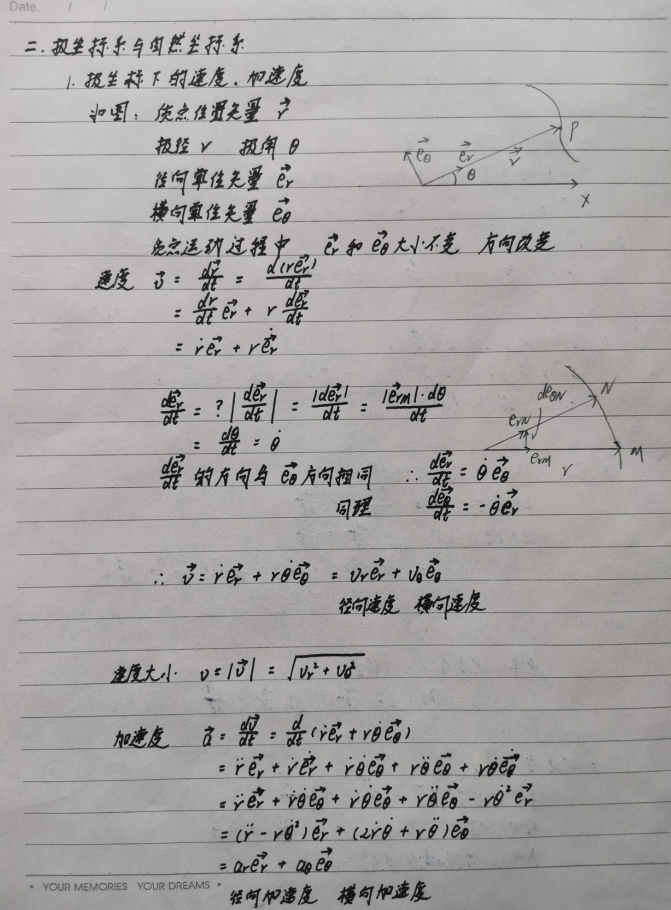
\includegraphics[width=13cm, height=18cm]{D:/UniversityNote/PhyNote/1.png}
\subsubsection{自然坐标下的速度,加速度}
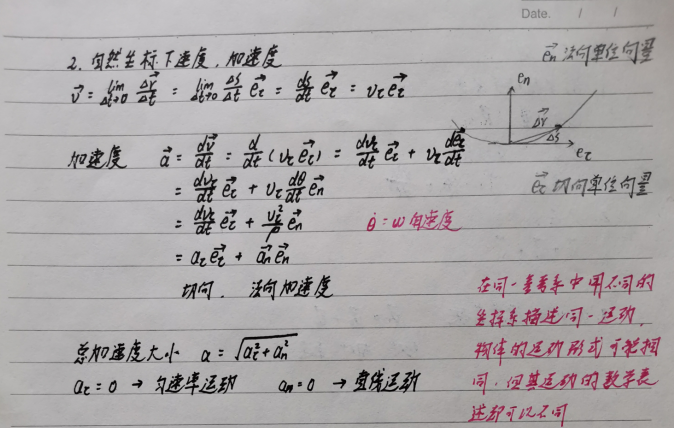
\includegraphics[width=13cm, height=10cm]{D:/UniversityNote/PhyNote/2.png}
\subsection{圆周运动的速度,角速度}
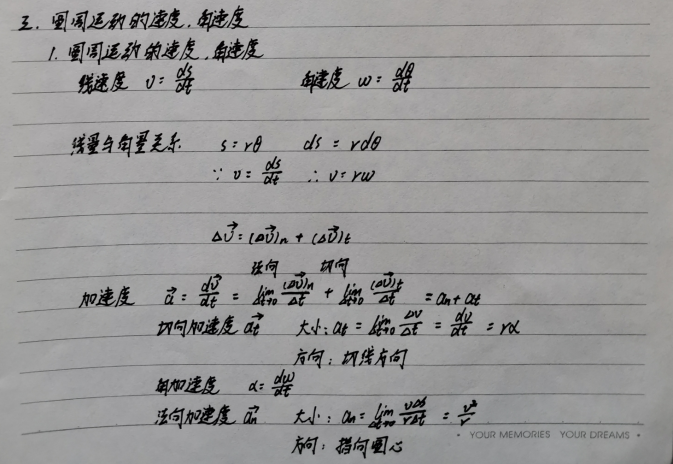
\includegraphics[width=13cm, height=10cm]{D:/UniversityNote/PhyNote/3.png}
\subsection{相对运动}
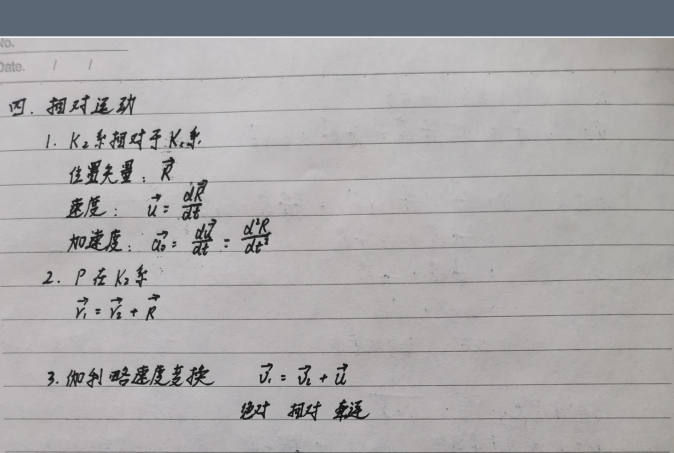
\includegraphics[width=13cm, height=10cm]{D:/UniversityNote/PhyNote/4.png}
\newpage
\section{第二讲\;\;牛顿运动}
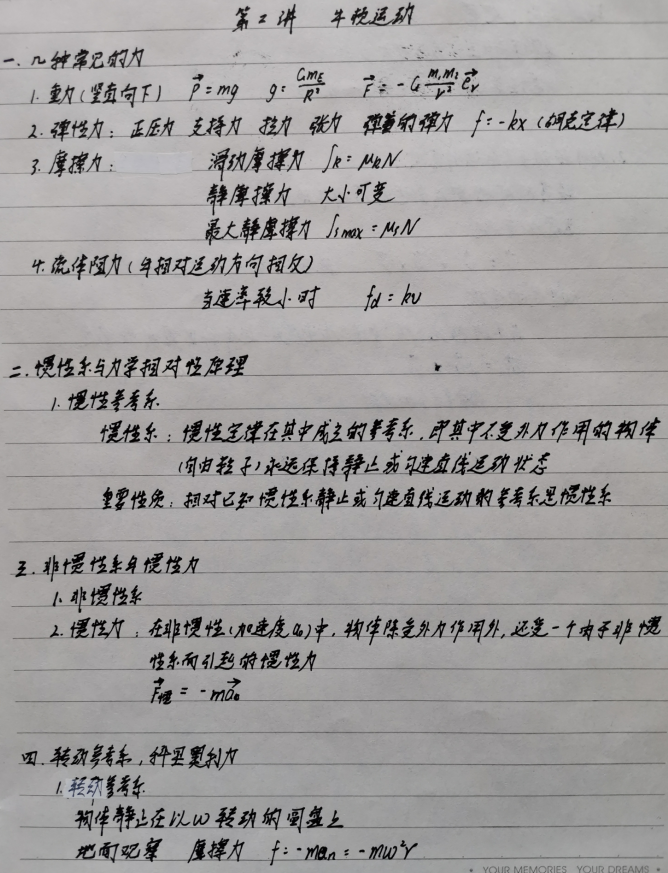
\includegraphics[width=13cm, height=18cm]{D:/UniversityNote/PhyNote/5.png}

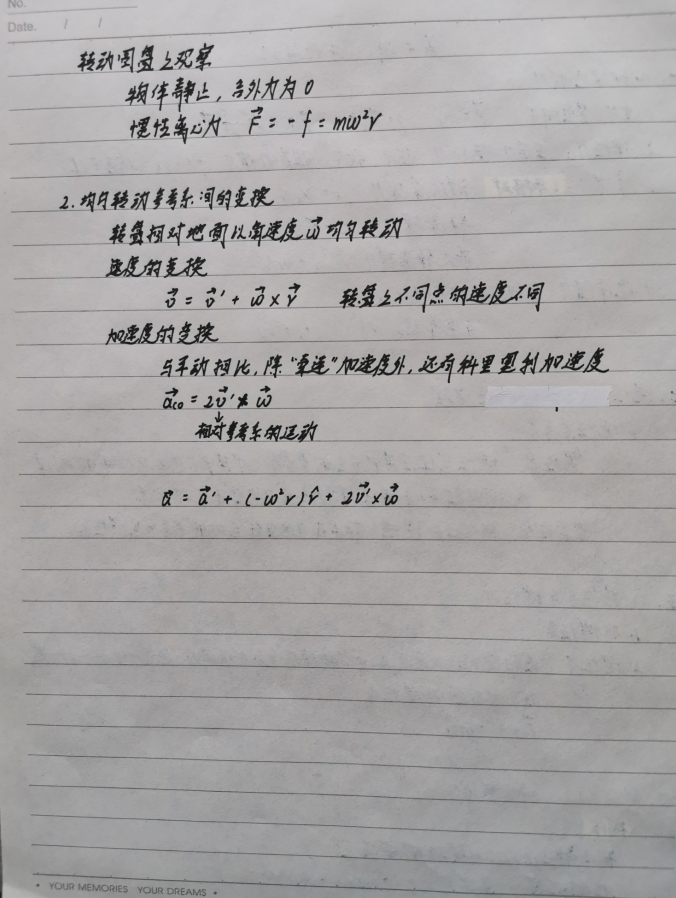
\includegraphics[width=13cm, height=18cm]{D:/UniversityNote/PhyNote/6.png}
\newpage
\section{第三讲\;\;动量定理\;\;动量守恒定律}
\subsection{质点动量定理}

    动量:$\vec{P} = m\vec{v}$,单位:$kg\cdot m/s$
    
    质点动量定理微分形式:$\vec{F}dt = d\vec{P}$

    质点动量定理积分形式:$\vec{I} = \int_{t_1}^{t_2}\vec{F}dt = \int_{P_1}^{P_2}d\vec{P} = \vec{p_2} - \vec{P_1}$

\subsubsection{质点动量定理}

    $\vec{I} = \vec{P_2} - \vec{P_1}$,过程量等于两状态量之差

    分量形式:$I_i = P_{2i} - P_{1i}\;(i = x, y, z)$,只适用于惯性系

\subsubsection{质点系动量定理}

    质点系内部n个质点,外部m个质点

    第i个质点所受力
    \[\vec{F_i} = \frac{d\vec{P_i}}{dt} = \sum_{\substack{i\neq j\\j=i}}^{m+n}\vec{F_{ij}}\;\;\;\;\;\vec{F_i} = \vec{F_{i\mbox{外}}}+\vec{F_{i\mbox{内}}}\]

    \[\vec{F_{i\mbox{外}}} = \sum_{\substack{i\neq j\\j=n+i}}^{m+n}\vec{F_{ij}}\;\;\;\;\;\vec{F_i} = \frac{d\vec{P_i}}{dt}\;\;\;\;\;\sum_{i+1}^n = \frac{d}{dt}\sum_{i+1}^n\vec{P_i}\]
    
    系统内力之和为零,质点系总动量\;\;$P = \sum_{i=1}^n\vec{P_i}$

    质点系动量定理:$\vec{F_{\mbox{外}}} = \frac{d\vec{P}}{dt}$\;\;\;系统受到的合外力等于系统动量对时间的变化率

    说明:内力能使系统内各个质点的动量发生改变(相互交换动量),但它们对系统的总动量没有任何影响

\subsubsection{动量守恒定律}

    由质点系动量定理\;\;\;$\vec{F_{\mbox{外}}} = \frac{d\vec{P}}{dt}$,当系统所受的合外力为0,即$\vec{F_{\mbox{外}}} = 0$

    \[\frac{d\vec{P}}{dt} = 0\;\;\;\;\;\vec{P} = \sum_i\vec{P_i} = \sum_im\vec{v_i}\;\;\mbox{常矢量}\]

    动量守恒定律:当一个质点系受到的合外力为零时,该系统的总动量保持不变

\subsection{质心,质心运动定理}

\subsubsection{质心}

    质心:\[\vec{r_c} = \frac{\sum_{i=1}^n m_i\vec{F_i}}{m}\;\;(m = \sum_i m_i)\]

    质心坐标:\[x_c = \frac{\sum_i m_i x_i}{m}\;\;\;y_c = \frac{\sum_im_iy_i}{m}\;\;\;z_c = \frac{\sum_im_ix_i}{m}\]

    质量连续分布的物体:\[r_c = \frac{\int\vec{r}dm}{m}\;\;\;x_c = \frac{\int xdm}{m}\;\;\;y_c = \frac{\int ydm}{dm}\;\;\;z_c = \frac{\int zdm}{m}\]

    说明:质心的定义与坐标原点的选择有关

\subsubsection{质心运动定理}

    由质心定义:$\vec{r_c} = \frac{\sum m_i\vec r_i}{m}$
    
    质心速度:$\vec{v_c} = \frac{d\vec{r_c}}{dt} = \frac{\sum m_i\vec{v_i}}{m}$

    质心加速度:$\vec{a_c} = \frac{d^2\vec{r_c}}{dt^2} = \frac{\sum_i m_i\vec{a_i}}{m}$

    质点系的动量是质点系内各质点动量的矢量和
    \[\vec{P} = \sum_i m_i\vec{v_i} = m\frac{\sum_i m_i\vec{v_i}}{m} = mv_c\]

    \[\vec{P} = m\vec{v_c}\;\;\;\;\;\vec{F_{\mbox{外}}} = \frac{d\vec{P}}{t} = m\frac{d\vec{v_c}}{dt} = m\vec{a_c}\;\;\;\;\;\vec{F_{\mbox{外}}} = m\vec{a_c}\mbox{——质心运动定理}\]

    当物体只做平动时,质心运动代表整个物体的运动

\subsection{碰撞}

    特点:相互作用时间短;冲击力大$\rightarrow$其它力相对很小$\rightarrow$只有内力$\rightarrow$整个系统动量守恒

    两球对心碰撞:$m_1\vec{v_{10}} + m_2\vec{v_{20}} = m_1\vec{v_1} + m_2\vec{v_2}$

    引入“恢复系数”:\[e = \lvert \frac{\vec{v_2} - \vec{v_1}}{\vec{v_{10}} - \vec{v_{20}}} \rvert\]

    可得\[v_1 = v_{10} - \frac{(1+e)m_2(v_{10} - v_{20})}{m_1 + m_2}\;\;\;v_2 = v_{20} + \frac{(1+e)m_1(v_{10} - v_{20})}{m_1 + m_2}\]

    完全弹性碰撞:$e = 1$;

    完全非弹性碰撞:$e = 0$;损失的机械能$\rightarrow$体系的内能

    非弹性碰撞:$0<e<1$;

\newpage
\section{第四讲\;\;动能定理\;\;功能原理}
\subsection{功\;\;功能定理}
\subsubsection{功}

    (1)物体作直线运动,恒力做功
    \[A = Fcos\theta \cdot \lvert \Delta \vec{r} \vert\;\;\;\;\;A = \vec{F}\cdot\vec{\Delta r}\]

    (2)物体作曲线运动,变力做功
    \[\mbox{元功:}dA = Fcos\theta\cdot\lvert d\vec{r}\vert = \vec{F}\cdot d\vec{r}\]

    \[\mbox{总功:}A = \int_A^BdA = \int_A^B\vec{F}\cdot d\vec{r} = \int_A^BFcos\theta \lvert d\vec{r}\vert\]

    (3)质点同时受几个力作用时

    力的叠加原理:$\vec{F} = \vec{F_1} + \vec{F_2} + \dots + \vec{F_N}$

    \;\;\;\;\;\;\;\;\;\;\;\;\;\;\;\;\;\;\;\;$A = A_{1AB} + A_{2AB} + \dots + A_{NAB}$

    说明:

    \;\;(1)合力的功等于各分力沿同一路径所做功的代数和

    \;\;(2)计算力对物体做功时,必须说明是哪个力对物体沿哪条路径所做的功

\subsubsection{动能定理}

    1、定义:质点动能\[E_k = \frac{1}{2}mv^2\mbox{ 或者 }E_k = \frac{p^2}{2m}\]

    2、质点的动能定理\[A_{\mbox{合}AB} = E_{kB} - E_{kA} = \Delta E_k = \frac{1}{2}mv_B^2 - \frac{1}{2}mv_A^2\]

    \;\;合外力对质点所做的功(其它物体对它所做的总功)等于质点动能的增量

    3、质点系动能定理

    对n个质点组成的质点系:对每个质点分别使用动能定理
    \[\sum_{i=1}^n A_{i\mbox{外}} + \sum_{i=1}^n A_{i\mbox{内} = \sum_{i=1}^n E_{kiB} - \sum_{i=1}^n E_{kiA}}\]

    所有外力对质点系做的功和内力对质点系做的功之和等于质点系总动能的增量

    注意:内力能改变系统的总动能,但不能改变系统的总动量

\subsection{保守力与非保守力}

    两质点间的“一对力”做功之和等于其中一个质点受的力沿着该质点相对于另一质点所移动的路径所做的功

    沿任意回路做功为零的力,或做功与具体路径无关的力都称为保守力

    大多数定向力和有心力都是保守力

\subsection{势能\;\;势能曲线}

    1、势能

    势能:系统在任一位形时的势能等于它从此位形沿任意路径改变至势能零点时保守力所做的功

    \[\mbox{势能}\left\{
        \begin{aligned}
        \mbox{势能与参考系无关(相对位移)     } \\
        \mbox{相对量:相对于势能零点的         } \\
        \mbox{系统量:是属于相互作用的质点共有的}
        \end{aligned}
        \right.\]
    
    \[\mbox{几种势能}\left\{
        \begin{aligned}
        \mbox{引力势能:(无穷远处为零势能点)} E_p(r) = -G\frac{m_1m_2}{r}\\
        \mbox{重力势能:(高度为零为零势能点)} E_p(h) = mgh\\
        \mbox{弹性势能:(自然伸长为零势能点)} E_p(x) = \frac{1}{2}kx^2
        \end{aligned}
        \right.\]
    
    2、势能曲线

    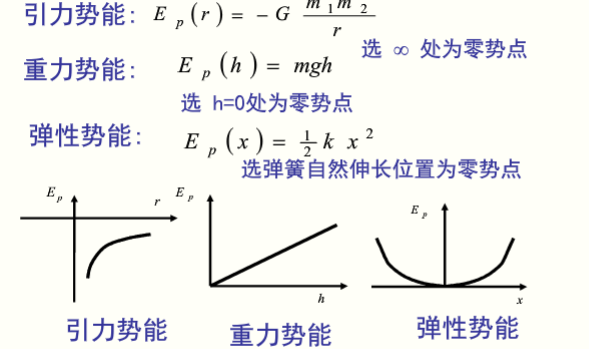
\includegraphics[width=13cm, height=8cm]{D:/UniversityNote/PhyNote/7.png}
    
    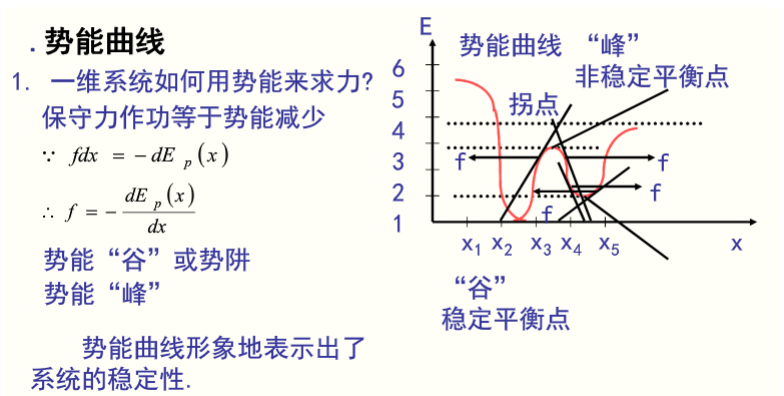
\includegraphics[width=13cm, height=8cm]{D:/UniversityNote/PhyNote/8.png}

    3、由势能求保守力

    梯度算符:$\bigtriangledown = \frac{\partial}{\partial x}\vec{i} + \frac{\partial}{\partial x}\vec{j} + \frac{\partial}{\partial x}\vec{k}$
    \[F_l = -\frac{dE_p}{dl}\;\;\;\;\;\vec{F} = -\bigtriangledown E_p\]

    保守力等于势能的负梯度

\subsection{功能原理以及机械能守恒定律}

    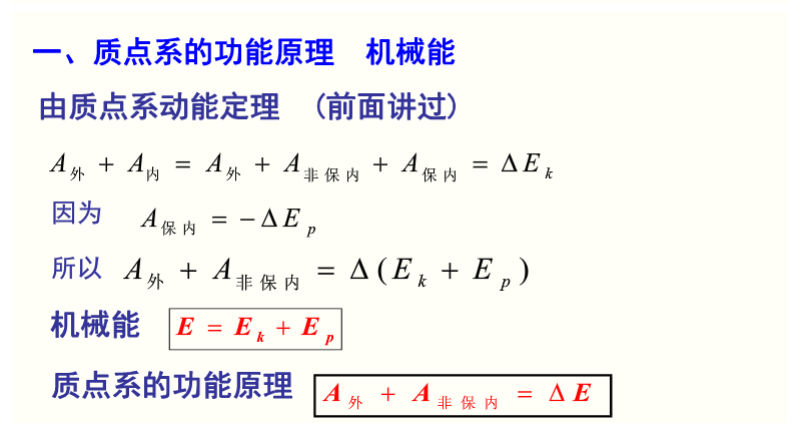
\includegraphics[width=13cm, height=8cm]{D:/UniversityNote/PhyNote/9.png}

    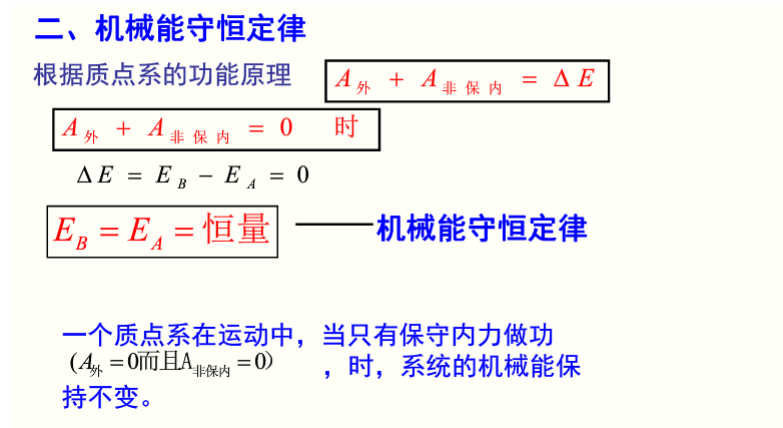
\includegraphics[width=13cm, height=8cm]{D:/UniversityNote/PhyNote/10.png}

\newpage
\section{第五讲\;\;角动量\;\;角动量守恒定律}
\subsection{质点的角动量}
\subsubsection{质点角动量的定义}

    质点的角动量是对某一固定参考点而言,t时刻质点对参考点O的角动量定义为:
    \[\vec{L} = \vec{r}\times\vec{P} = \vec{r}\times m\vec{v}\]

    角动量的大小:$L = rmvsin\phi$,单位:$kg\cdot m^2/s$或$J\cdots$

    方向:服从右手螺旋法则,垂直于$\vec{r},\vec{P}$所在的平面

    说明:

    (1)角动量是瞬时量

    (2)质点动量为零,角动量必为零;动量不为零,角动量也可能为零

    (3)匀速率圆周运动时,相对于圆心的角动量为$L = Rmv$;动量改变,角动量恒定

    (4)统一运动质点,参考点选择不同,角动量不同

\subsection{质点角动量定理及守恒定律}
\subsubsection{质点角动量定理}

    质点对参考点O的角动量:$\vec{L} = \vec{r}\times\vec{P}$

    上式取时间的微分:
    
    $\frac{d\vec{L}}{dt} = \frac{d}{dt}(\vec{r}\times\vec{P}) = \frac{d\vec{r}}{dt}\times\vec{P} + \vec{r}\times\frac{d\vec{p}}{dt} = \vec{v}\times m\vec{v} + \vec{r}\times\vec{F} = \vec{r}\times\vec{F}$

    质点角动量定理:\[\frac{d\vec{L}}{dt} = \vec{M}\]

    质点角动量定理变形为$\vec{M}dt = d\vec{L}$,对$t_1\rightarrow t_2$时间过程,有
    \[\int_{t_1}^{t_2}\vec{M}\cdot dt = \vec{L_2} - \vec{L_1}\]

    质点对固定点角动量的增量等于该质点所受合力的冲量矩

\subsubsection{力对固定轴的力矩}

    (1)角动量和力矩均与参考点有关,角动量也称动量矩,力矩也叫角力

    (2)角动量的分量形式也成立:
    
    $\vec{L} = \vec{r}\times\vec{P} = L_x\vec{i} + L_y\vec{j} + L_Z\vec{k}\;\;\;\vec{M} = \vec{r}\times\vec{F} = M_x\vec{i} + M_y\vec{j} + M_z\vec{k}$

    即:$\frac{dL_x}{dt} = M_x\;\;\;\frac{dL_y}{dt} = M_y\;\;\;\frac{dL_z}{dt} = M_z$

    (3)对轴的角动量和对轴的力矩,再具体的坐标系中,角动量(或力矩)在某一坐标轴上的分量,称质点对该轴的角动量(或力矩)

\subsubsection{质点角动量守恒定律}

    若对某一固定点,质点所受和力矩为零,则质点对该固定点的角动量矢量保持不变————质点角动量守恒定律

    (1)$\vec{M} = 0$的条件是:$\vec{F} = 0\;\;\;\;\;\vec{F}$过固定点:有心力

    (2)动量守恒,角动量一定守恒;动量不守恒,角动量也可能守恒

    (3)角动量的分量形式亦成立

\subsection{质点系的角动量定理及其守恒定律}
\subsubsection{质点系的角动量定理}

    质点系中各个质点对某一固定点的角动量的矢量和,即为该质点系对该固定点的角动量\[\vec{L} = \sum_i\vec{L_i} = \sum_i\vec{r_i}\times\vec{p_i}\]

    由质点角动量定理可知\[\frac{d\vec{L_i}}{dt} = \vec{M_i} = \vec{r_i}\times(\vec{F_i}+\sum_{j\neq i}\vec{f_{ij}})\]即\[\frac{d\vec{L}}{dt} = \sum_i\frac{d\vec{L_i}}{dt} = \sum_i\vec{r_i}\times\vec{F_i} + \sum_i(\vec{r_i}\times\sum_{i\neq j}\vec{f_{ij}}) = \vec{M_{\mbox{外}}} + \vec{M_{\mbox{内}}}\]

    又\[\vec{r}\times\vec{f_{if}} + \vec{r_j}\times\vec{f_{ji}} = (\vec{r_i} - \vec{r_j})\times\vec{f_{ij}} = 0\;\;\;\;\;\mbox{即}\;\vec{M_{\mbox{内}}} = 0\]

    于是\[\vec{M_{\mbox{外}}} = \frac{d\vec{L}}{dt}\]

    一个质点系所受的合外力矩等于该质点系的角动量对时间的变化率————质点系的角动量定理

\subsubsection{质点系的角动量守恒定律}

    (1)质点系的角动量定理也是适用于惯性系
    (2)外力矩和角动量都是相对于惯性系中的同一固定点说的
    (3)当合外力矩为零时,质点的角动量不随时间变化————质点系的角动量守恒定律
    (4)内力矩不影响质点系总角动量,但影响质点系中某些质点的角动量

\subsection{刚体模型及其运动}

    1、刚体的定义:在力的作用下,形状与体积都不变的物体称为刚体

    2、刚体的特点:刚体是特殊的质点系,组成刚体的各个质元之间的相对位置保持不变,刚体是理想化模型,物体的形变远小于其本身的限度,在描述其运动时可抽象为刚体

\subsubsection{刚体的运动}

    1、平动:刚体内任意两质元连线在运动过程中始终保持平行

    2、平动的特点:运动学范畴内,平动的刚体可视为质点,可用质点运动学描述其运动,平动刚体的运动轨迹可以是三维的

    3、转动:刚体的各质元都绕某一直线(转轴)做圆周运动

    \begin{tabular}{|c|c|}% 通过添加 | 来表示是否需要绘制竖线
        \hline  % 在表格最上方绘制横线
        转轴固定&转轴方向不固定)\\
        \hline  %在第一行和第二行之间绘制横线
        定轴转动(纯转动&定点转动(轴上某点静止)\\
        \hline % 在表格最下方绘制横线
    \end{tabular}

    4、定轴转动特点:定轴转动的刚体中各质元在各自的转动平面内绕轴作不同半径的圆周运动

    5、一般运动:一般运动 = 随基点的平动 + 绕基点的定轴转动,转动大小与基点(质心)的选取无关

\subsection{刚体定轴转动的运动描述}

    定轴转动的刚体中任意质元都在各自的转动平面内,以一定的转动半径做圆周运动

\subsubsection{定轴转动的角量描述}

    1、角位置:$\theta = \theta (t)$,沿逆(顺)时针方向转动\;\;\;$\theta >(<) 0$

    2、角位移:$\Delta\theta = \theta(t + \Delta t) - \theta(t)\;\;\;\Delta\theta$的方向:由右手螺旋确定

    3、角速度:$\omega = \frac{d\theta}{dt}\;\;$角速度的方向可用正负来表示

    4、角加速度:$\beta = \frac{d\omega}{dt}\;\;$反向:越转越快(慢)时,与$\vec{\omega}$同(反)方向

    刚体上所有质元都具有相同的角位移,角速度,角加速度

    定轴转动的描述仅需一维(角)的坐标

    5、匀变速转动:刚体绕定轴转动的角速度为恒量时,刚体做匀速转动,绕定轴转动的角加速度为恒量时,刚体做匀变速运动

    刚体匀变速转动与质点匀变速直线运动公式对比

    \begin{tabular}{|c|c|}% 通过添加 | 来表示是否需要绘制竖线
        \hline  % 在表格最上方绘制横线
        质点匀变速直线运动&刚体绕定轴做匀变速转动\\
        \hline  %在第一行和第二行之间绘制横线
        $v = v_0 + at$&$\omega = \omega_0 + \beta t$\\
        \hline % 在表格最下方绘制横线
        $x = x_0 + v_0t + \frac{1}{2}at^2$&$\theta = \theta_0 + \omega_0t + \frac{1}{2}\beta t^2$\\
        \hline % 在表格最下方绘制横线
        $v^2 = v_0^2 + 2a(x - x_0)$&$\omega^2 = \omega_0^2 + 2\beta(\theta - \theta_0)$\\
        \hline % 在表格最下方绘制横线
    \end{tabular}

\subsubsection{定轴转动角量和线量大小的关系}

    \[s = R\theta\;\;\;\;\;\Delta s = R\Delta\theta\]

    \[v = \frac{ds}{dt} = R\frac{d\theta}{dt} = R\omega\;\;\;\;\;a_\tau = \frac{dv}{dt} = R\frac{d\omega}{dt} = R\beta\;\;\;\;\;a_n = \frac{v^2}{R} = \frac{(R\omega)^2}{R} = R\omega^2\]
\subsection{刚体的转动惯量}
\subsubsection{转动惯量的定义}

    定轴转动的刚体,各质元到转轴距离的平方与质量乘积的总和,称为刚体对该转轴的转动惯量

    质量不连续分布:$J = \sum_i \Delta m_ir_i^2$

    质量连续分布:$J = \int r^2dm$

    转动惯量是标量\;\;\;\;\;[SI]:$kg\cdot m^2$

    转动惯量的意义:反映了刚体转动惯性的大小

\subsubsection{转动惯量的特点}

    与刚体总质量有关,与刚体质量分布有关,与转轴的位置有关

\subsubsection{有关转动惯量的几个定理}

    (1)转动惯量叠加原理:对于多个刚体组成的体系而言,相对某一固定轴的转动惯量等于每个刚体对该轴的转动惯量之和$J_z = J_A + J_B + J_C$

    (2)平行轴定理:如果已知质量为m的刚体绕通过其质心的某一个轴的转动惯量为$J_c$,则它相对于其质心轴平行、且相距为d的另一个轴的转动惯量为$J_z = J_c + md^2$

\subsection{力矩}
\subsubsection{力对固定点的力矩}

    力$\vec{F}$对参考点0的力矩:\[\vec{M} = \vec{r}\times\vec{F}\]

    大小:$\lvert \vec{r}\times\vec{F}\rvert = Frsin\theta = Fd$

    方向:右手螺旋法则

    说明:

    \;\;\;(1)质点不受力作用,力矩一定为零;力不为零时,力矩可能为零

    \;\;(2)力作用于参考点或其作用线通过参考点时,力对参考点的力矩为零

    \;\;(3)力矩的作用效果是产生相对于参考点O的转动状态

\subsubsection{力对固定轴的力矩}

    力对转轴z的力矩$\vec{M_z} = \vec{r}\times\vec{F_{\bot}}$

    力对轴的力矩的实质是力对O点的力矩在z轴方向上的分量

    对轴力矩大小:$M_z = \pm\lvert\vec{M_z}\rvert = \pm\lvert\vec{r}\times\vec{F_{\bot}}\rvert = \pm F_{\bot}rsin\theta = \pm F_{\bot}d$

    若$\vec{M_z}$沿规定的正方向,取“+”,反之,取“-”

    力矩叠加原理:当几个力矩作用在同一刚体上时,合力矩M时各单个力矩之和

    住:力矩求和只能对同一参考带点(或轴)进行

\subsection{刚体定轴转动定律}

    刚体定轴转动定律:\[M = J\beta\]

    刚体定轴转动的角加速度与它所受合外力矩成正比,与刚体的转动惯量成反比

    说明:

    \;\;\;(1)刚体所受力矩一定的情况下,转动惯量越大,角加速度越小

    \;\;(2)转动惯量是刚体转动惯性大小的量度

\subsection{定轴转动刚体角动量定理及其守恒定律}
\subsubsection{定轴转动刚体角动量定理}

    绕定轴转动的刚体的角动量:$L_z = J_z\omega$

    定轴转动刚体为质点系,满足质点系的角动量定理:$\vec{M_{\mbox{外}}} = \frac{d\vec{L}}{dt}$

    则有定轴转动角动量定理:\[M_z = \frac{dL_z}{dt} = \frac{d}{dt}(J_z\omega)\]

    定轴转动角动量定理积分形式:\[\int_{t_1}^{t_2}M_zdt = J_z\omega_2 - J_z\omega_1\]

\subsubsection{定轴转动刚体角动量守恒定律}

    刚体绕定轴转动时,如果所受合力矩为零,则刚体沿该轴的角动量守恒,此时,定轴转动刚体匀速转动

    当$M_z = 0$时,$J_z\omega=$恒量(大小不变,正负不变)

    刚体系:$M_z = 0$时,$\int J_{iz}\omega_i = const$

    角动量可在系统内部各刚体间传递,而却保持刚体系对转轴的总角动量不变

\subsection{刚体定轴转动动能和动能定理}

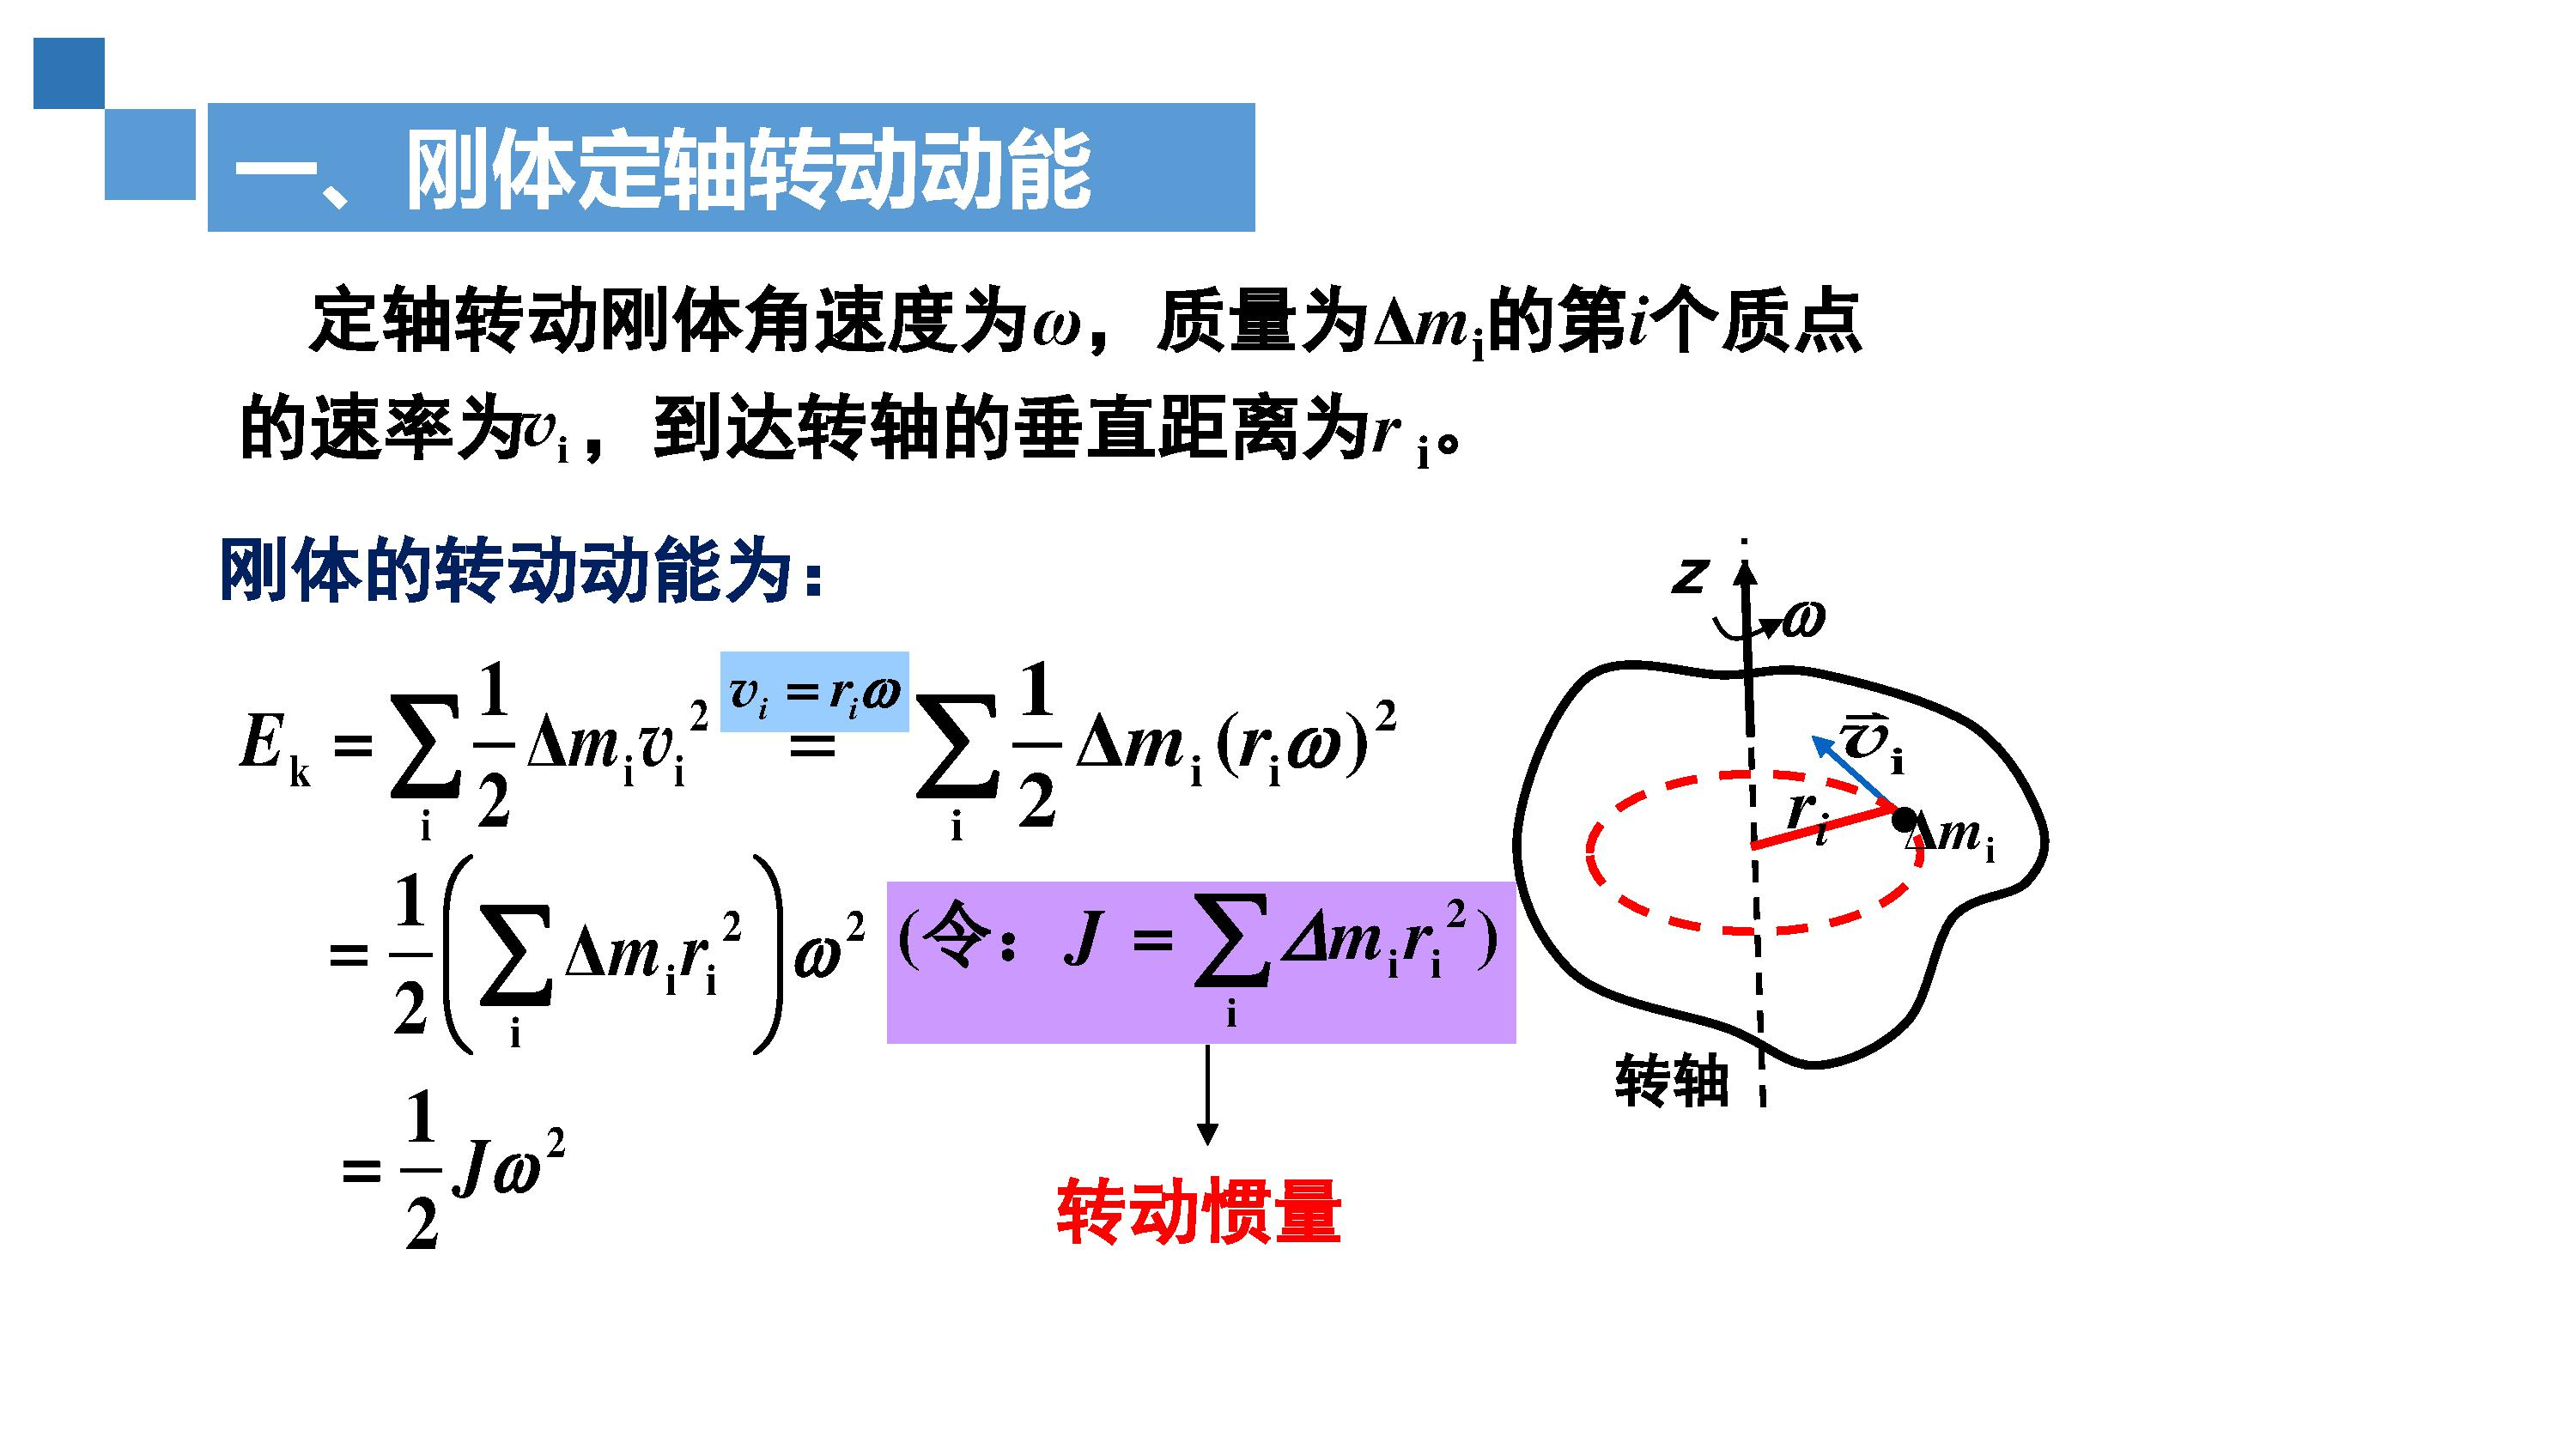
\includegraphics[width=13cm, height=8cm]{D:/UniversityNote/PhyNote/5102.jpg}

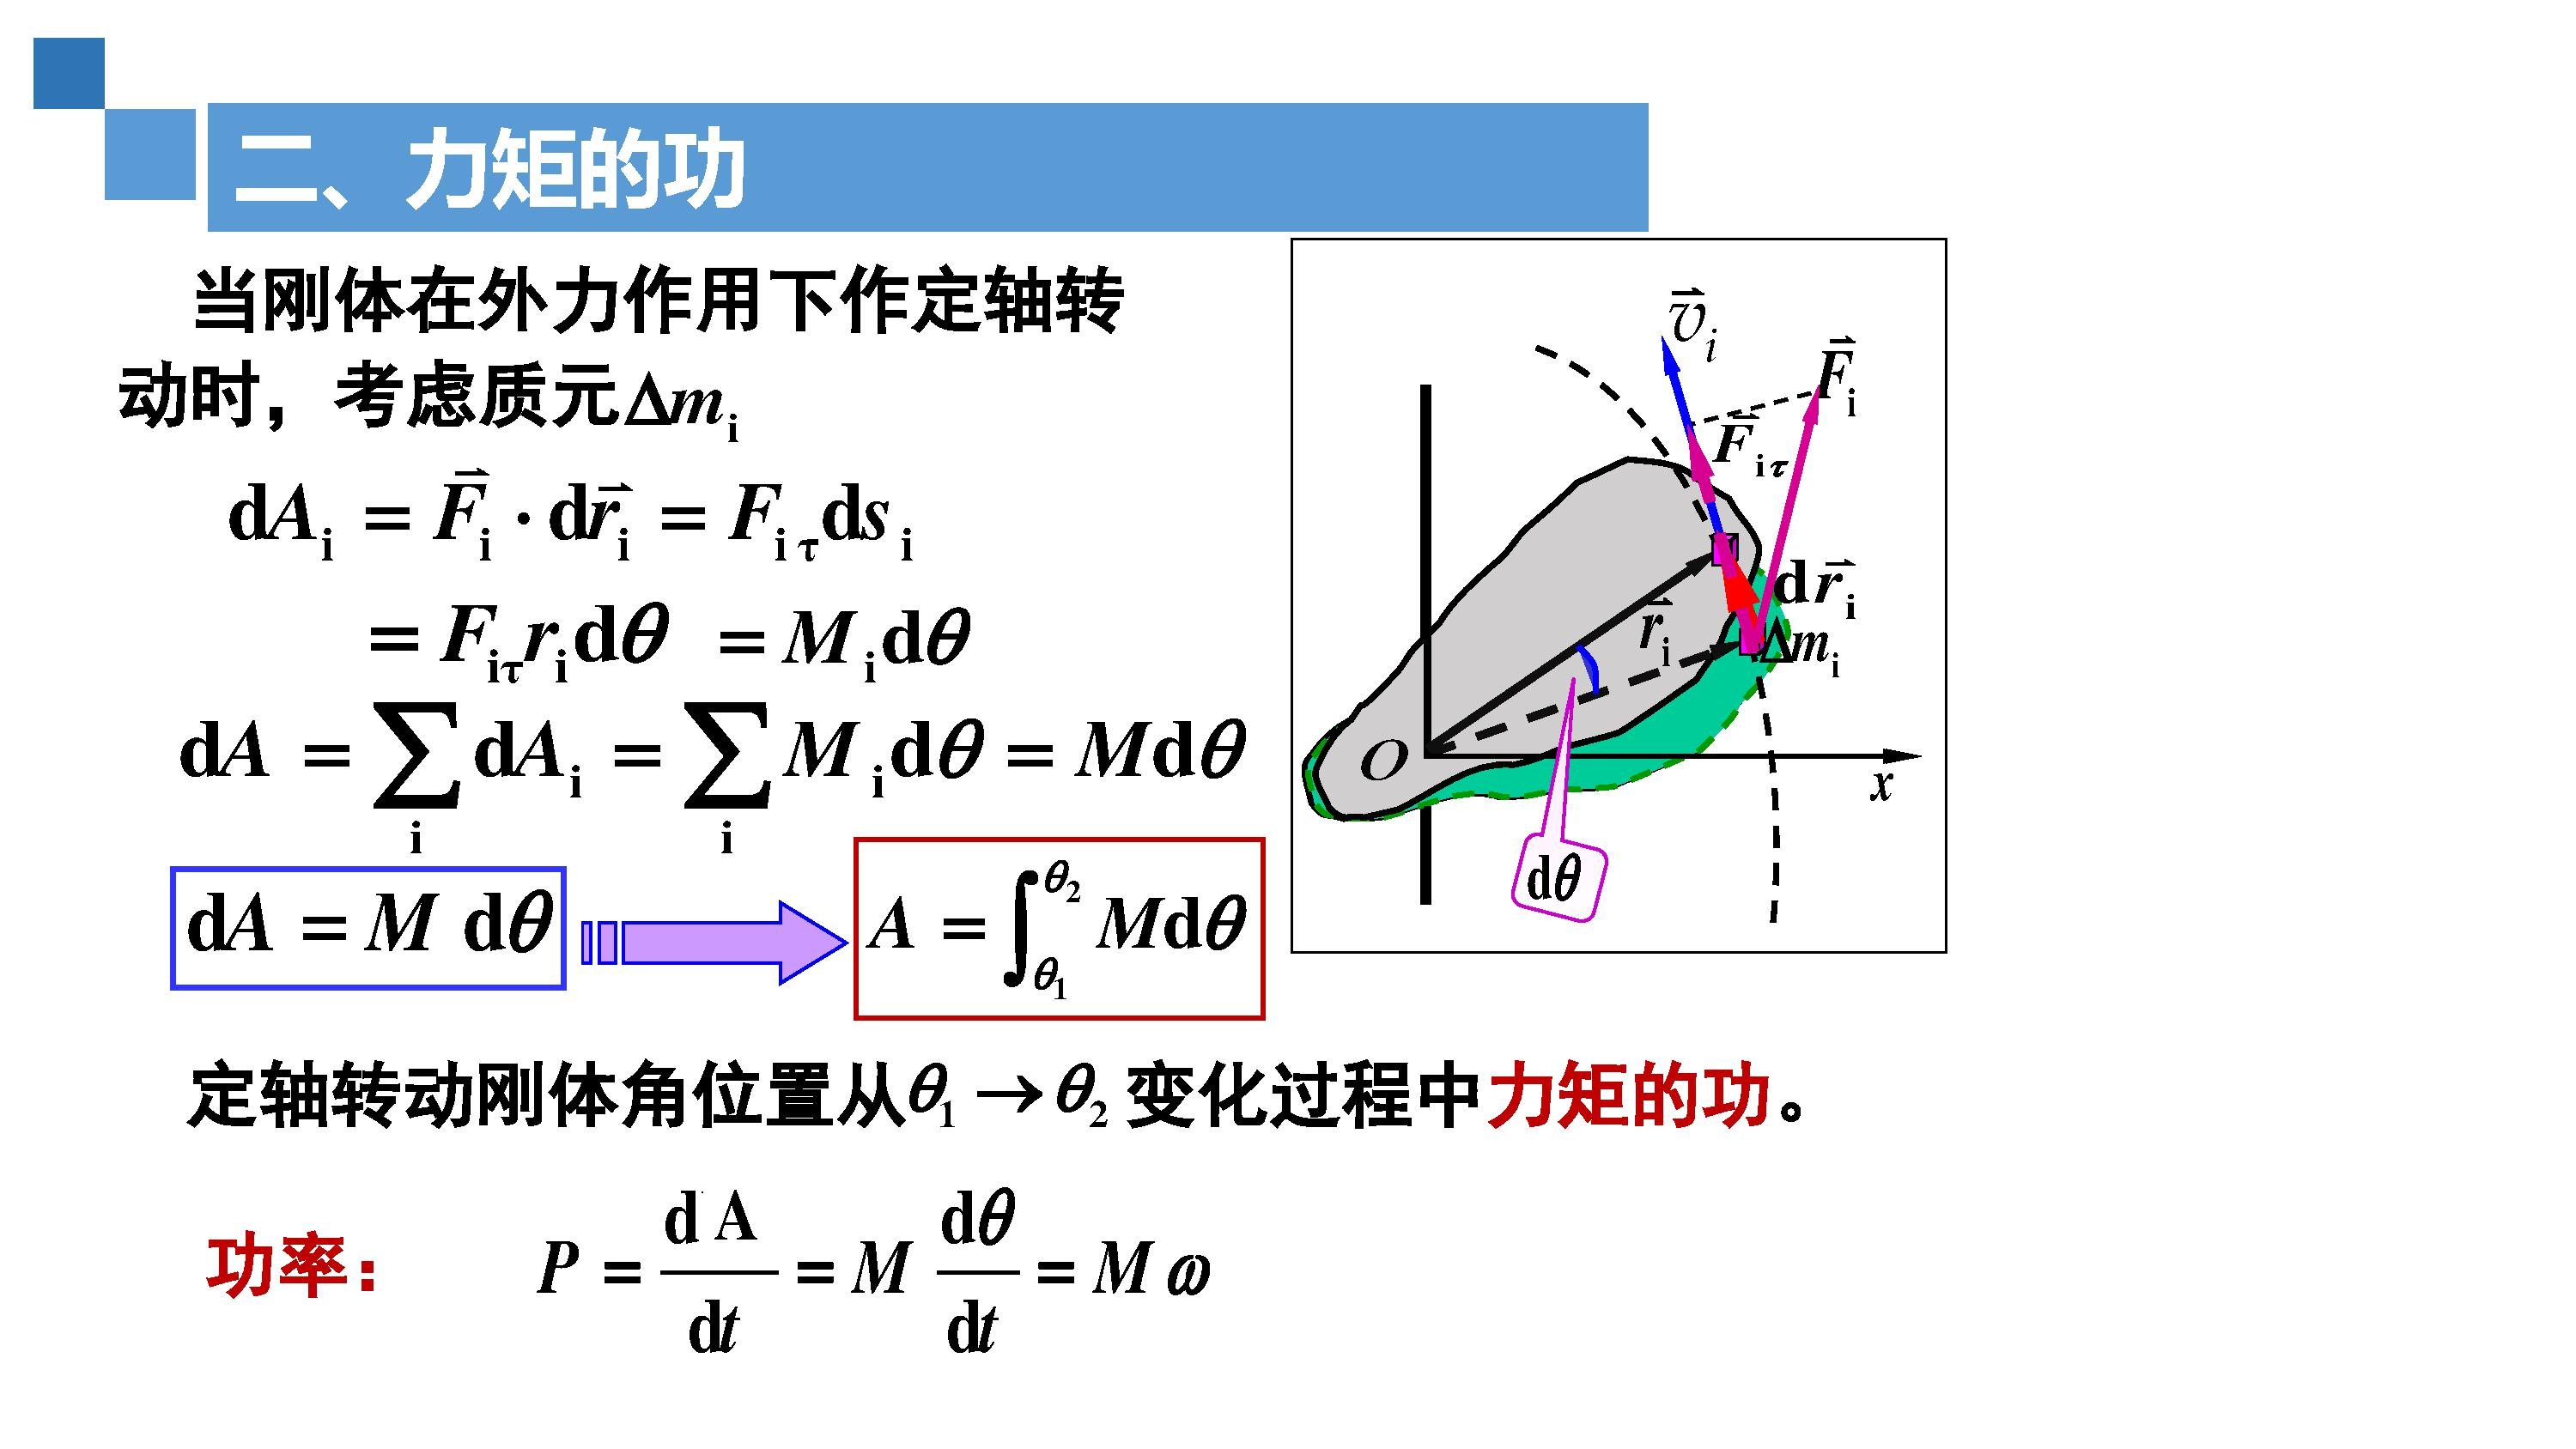
\includegraphics[width=13cm, height=8cm]{D:/UniversityNote/PhyNote/5103.jpg}

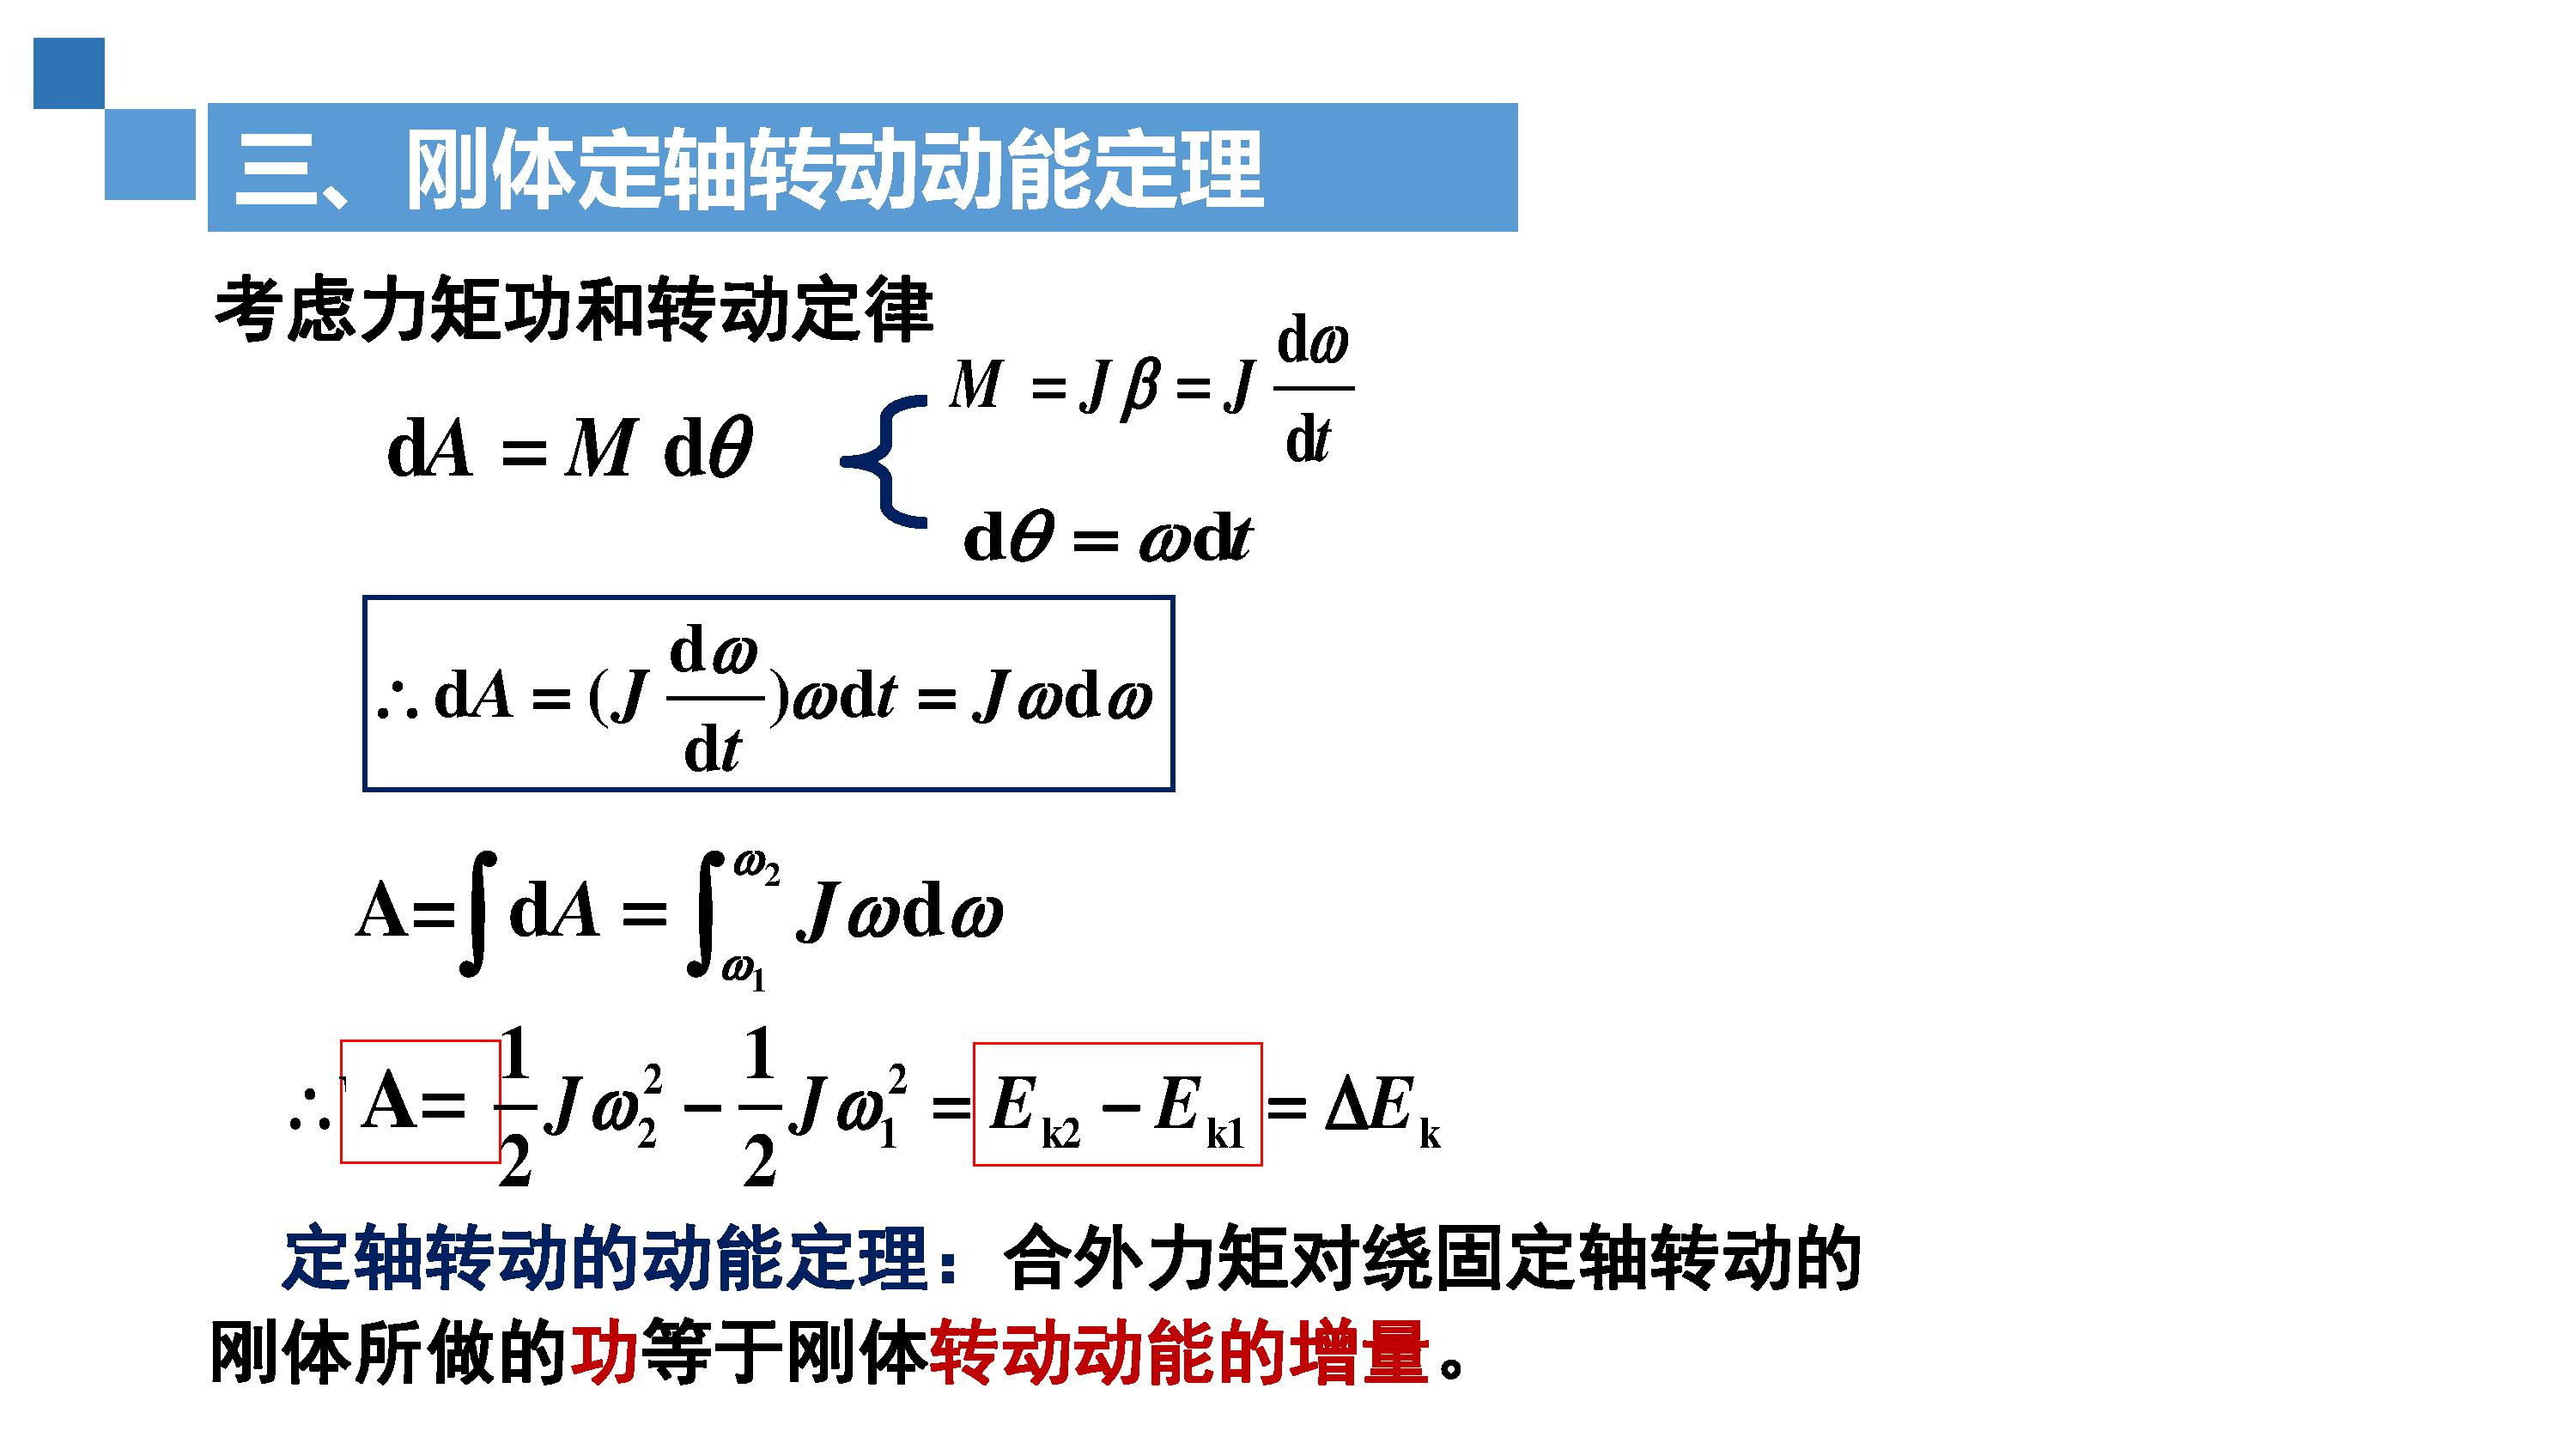
\includegraphics[width=13cm, height=8cm]{D:/UniversityNote/PhyNote/5104.jpg}

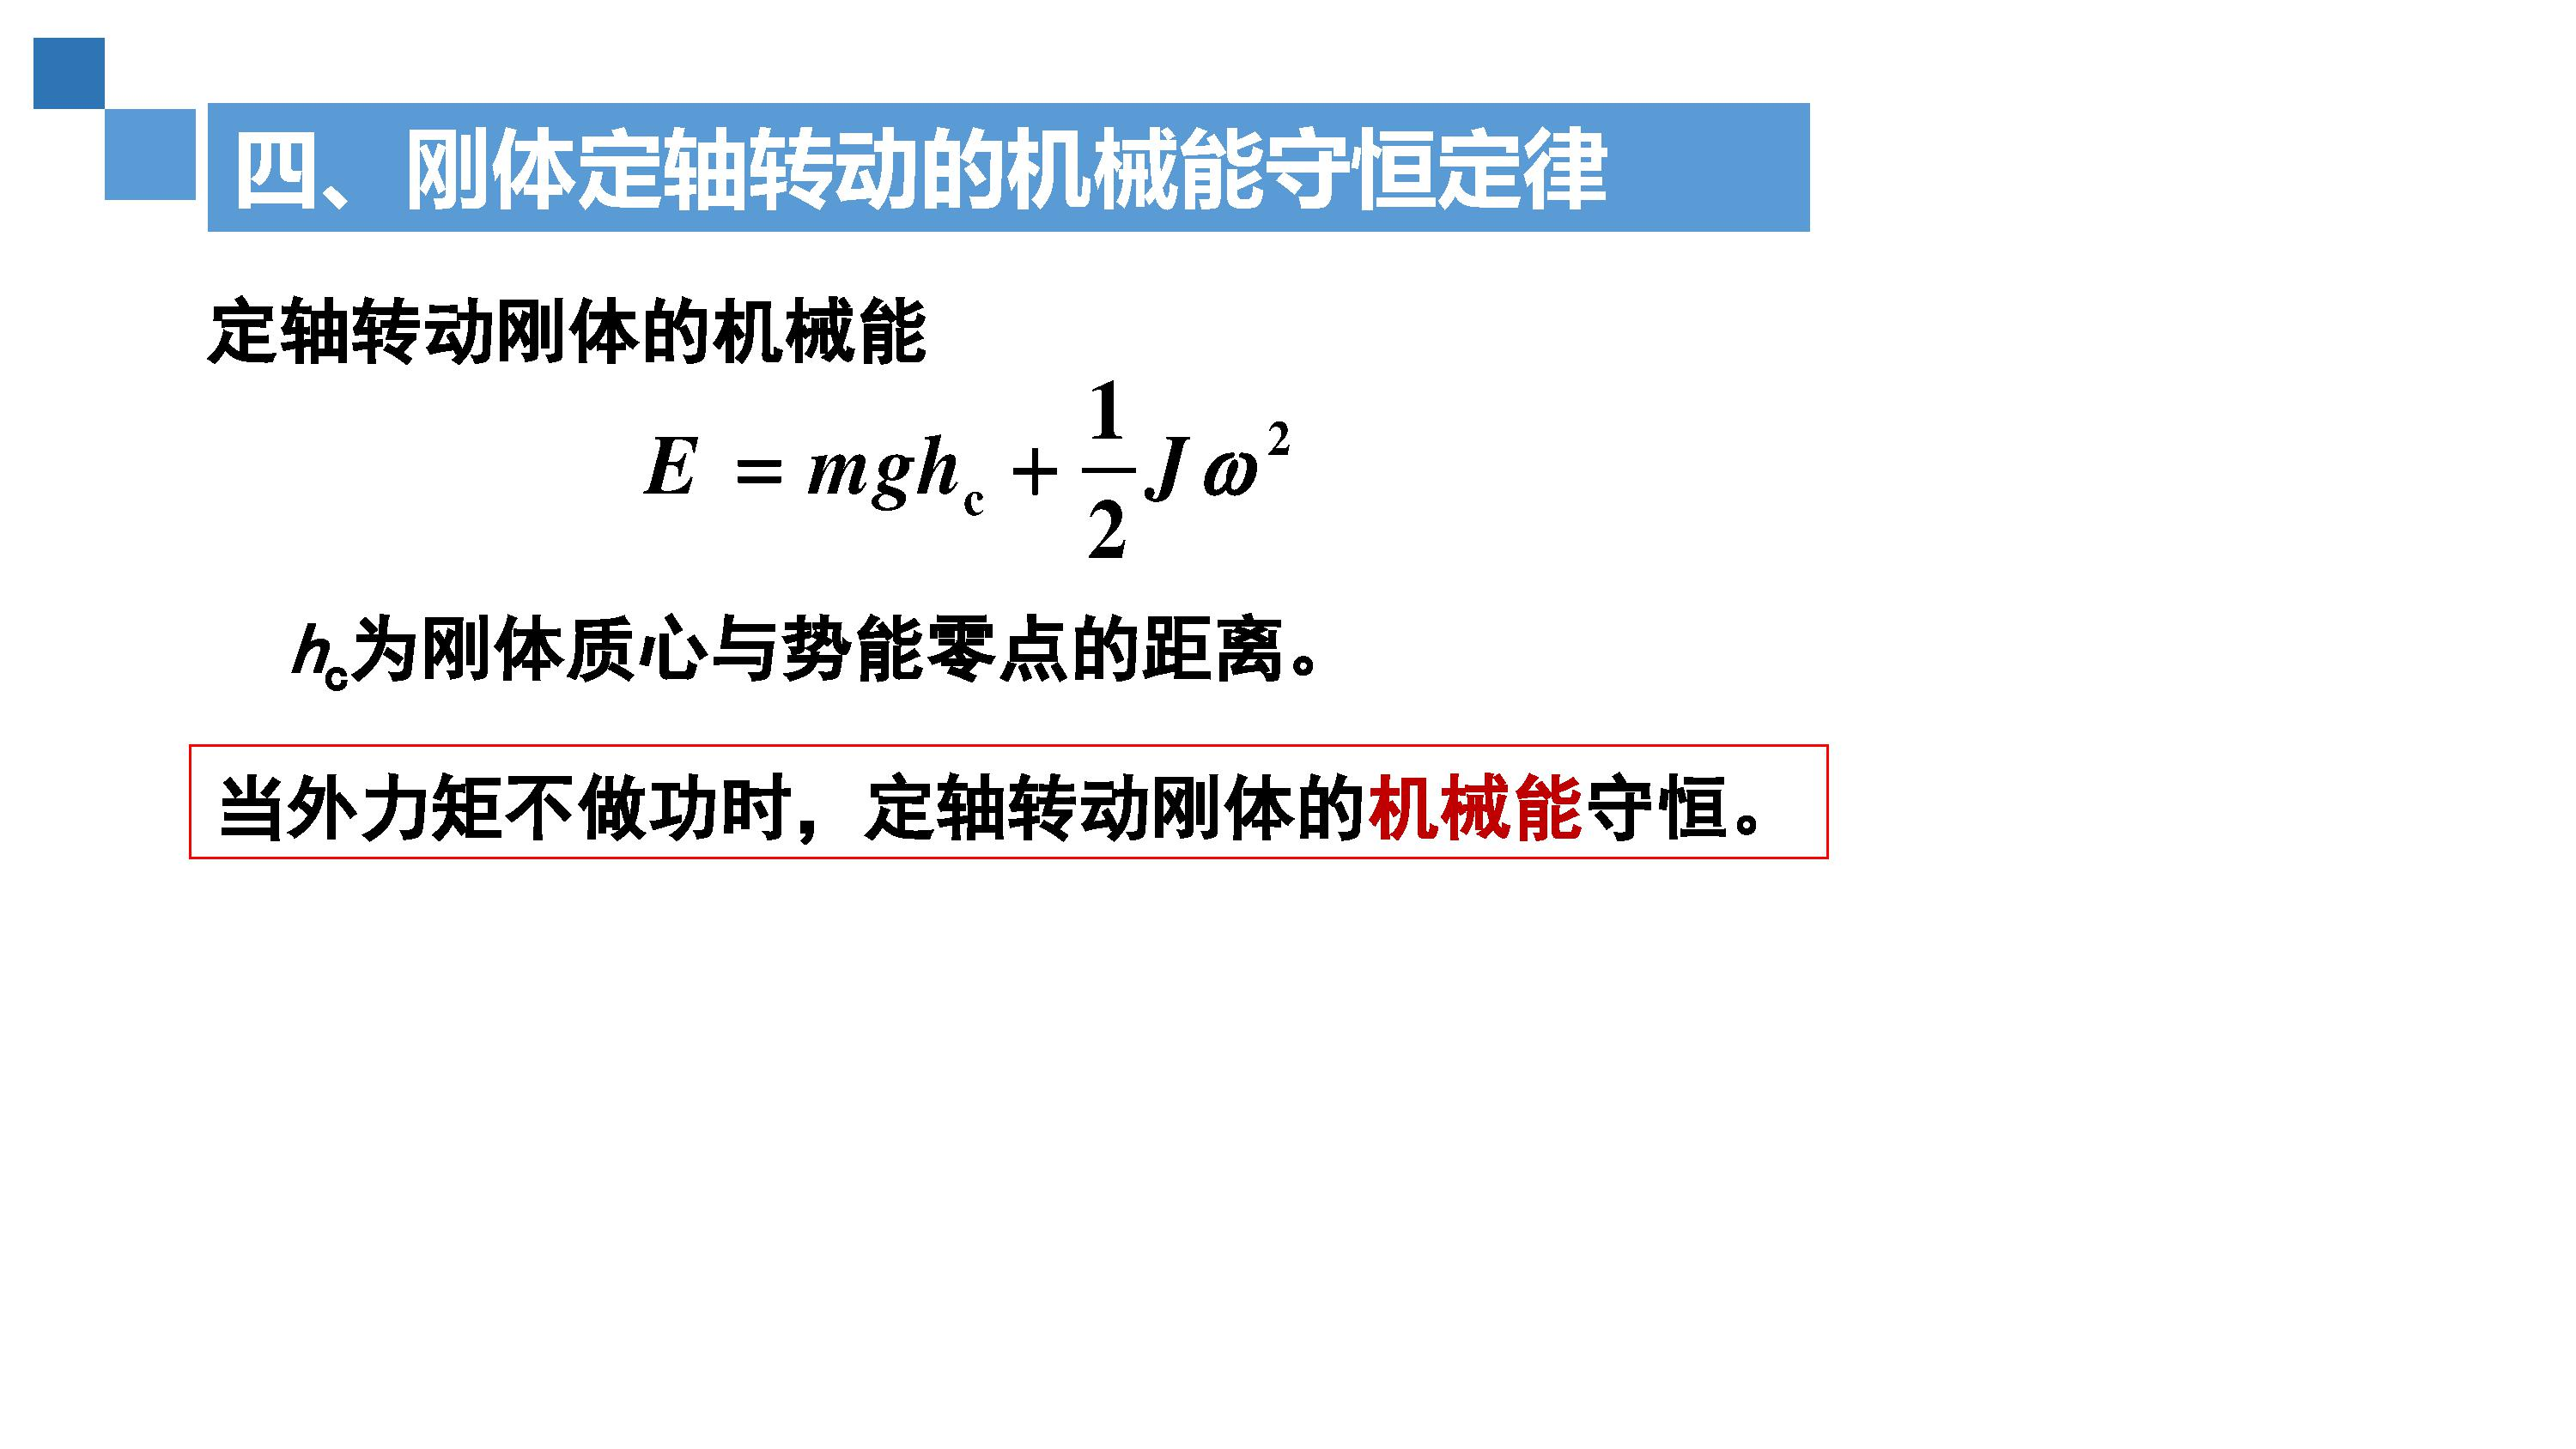
\includegraphics[width=13cm, height=8cm]{D:/UniversityNote/PhyNote/5105.jpg}
\newpage
\section{第六讲\;\;流体力学}
\subsection{压强与平衡方程}

    物质的三态:固态,液态,气态

    流体(液态,气态):具有一定体积、无固定形状、易于变形,具有一定的流动性

    液体和气体的不同点:液体有一定体积,几乎不可压缩,黏性大;气体没有一定体积,充满整个容器,易压缩,粘性小

    连续介质假设:流体在其存在的空间是连续、无间隙分布的,可取微分元

    流体元:宏观足够小而微观足够大,流体物理量是大量流元的相应物理量的统计平均

\subsubsection{流体静力学压强}

    静止流体没有抵抗剪切形变的能力,作用在流体内任一面元上的应力必与该面元垂直

    在静止流体中任取一个小面元$d\vec{s}$,作用在此面元上的力为$d\vec{f}$

    $\mbox{通常流体内部的压力:}d\vec{f} = -pd\vec{s}$

    p称为流体静力学压强,p为标量,单位帕(Pa)

    流体中静压强与面元取向无关

\subsubsection{静止流体的平衡方程}

    作用在流元上的力可以分为两类

    面积力:可用压强表述,作用在流元外表面上

    体积力:作用在每一质量微元上,亦称质量力

    设单位质量流体上的体积力为$\vec{F}$,则$d\vec{F} = \rho \vec{F}dxdydz$

    对静止流体:$\rho \vec{F}dxdydz - \bigtriangledown pdxdydz = 0$

    即\[\rho \vec{F} = \bigtriangledown p\;\;\;\rho F_x = \frac{\partial p}{\partial x}\;\;\;\rho F_y = \frac{\partial p}{\partial y}\;\;\;\rho F_y = \frac{\partial p}{\partial z}\]

    结论:体积力与压强梯度方向平行,体积力与等压面垂直

    重力场中的静止流体\[\frac{\partial p}{\partial x} = 0\;\;\;\frac{\partial p}{\partial y} = 0\;\;\;\frac{\partial p}{\partial z} = -\rho g\]

    设深度$z = z_A$处的压强$p_A$,$z = z_B$处的压强$p_B$,若密度为常量
    \[p_B = p_A - \int_{z_A}^{z_B}\rho gdz = p_A - \rho g(z_B - z_A)\]

    静止在重力场中的同种流体

    \;\;(1)液体中压强随距液面深度线性变化

    \;\;(2)等压面是水平面,与重力方向垂直

    \[\frac{dp}{dz} = -\rho g\;\;\;\;\;z + \frac{p}{\rho g} = c\mbox{(常数)}\]

\subsection{流体连续性原理}

    流体的粘性:流体流动时,各流层间存在着阻碍相对运动的内摩擦力,这就是流体的粘性。

    理想流体:不可压缩、无粘性的流体称为理想流体

\subsubsection{流体运动的描述方法}

    1.拉格朗日法:以研究个别流元的运动为基础,通过对每个流元运动规律的研究来获得整个流体的运动规律。
    (着眼于流体质点,跟踪每个流元来了解整个流体的运动规律。)

    2.欧拉法:考察通过空间固定的位置点的不同液体质点的运动状态,形成一个矢量场来了解流体在整个运动空间内的流动情况。
    (着眼于空间点,研究流经空间各固定点的流元的运动,获取流体的运动规律。)

    任一时刻流体空间的每一点上都有一个流速$\vec{v}$与之对应,形成一个矢量场—流速场。如果流速只是空间坐标的函数而不依赖于时间,则称为稳定流动,简称稳流。

    迹线:某一流体质点在运动过程中,不同时刻所流经的空间点连成的曲线。

    流线:某瞬间在流场中绘出的曲线,曲线上各流元的速度矢量和该线相切
    
    (1)流线表示瞬时流动方向,流线不能相交。
    
    (2)流线密处流速大,流线稀处流速小

    流管:某时刻在速度场中做一条非流线的曲线,经过曲线上的每一点做流线,这些流线在空间形成一个曲面,称为流面。如果在流体中所做的非流线的曲线是闭合的,则所得到的流面称为流管。流管内外的流体都没有穿过流面的速度分量,管内流体不能流到管外,管外流体也不能流入管内。对稳定流动,流线和流管都不随时间变化,流管和真的管道相似。
    
\subsubsection{流体的连续性原理}

    体积流量:流体中单位时间内流过某一横截面的流体体积

    对于面元$\Delta \vec{s} \rightarrow 0\;\;\;\Delta \vec{s}\rightarrow d\vec{s}$
    
    可认为面元上各点流速$\vec{v}$相等,单位时间内流过面元的流体体积
    \[dQ_v = \frac{dV}{dt} = \frac{ds\cdot vdt\cdot cos\theta}{dt} = \vec{v}\cdot d\vec{s}\]

    对一封闭曲面S$Q_V = \int dQ_V = \int_S\vec{v}\cdot d\vec{s}$——体积流量

    质量流量:流体中单位时间内流过某一横截面的流体质量$dQ_m = \rho \vec{v}\cdot d\vec{s}\;\;\;Q_m = \int dQ_m = \int_S\rho\vec{v}\cdot d\vec{s}$

    流体的连续性原理:$\rho \vec{v}\cdot d\vec{s} - \int_S\frac{\partial \rho}{\partial t}dV = 0$

    不可压缩流体:$\frac{\partial \rho}{\partial t} = 0\;\;\;\int_S\vec{v}\cdot d\vec{s} = 0$

    稳定流动:流管不随时间变化,类似真实管道

    稳定流动的连续性原理:

    \;\;对任意流管:$\rho vdS = $常量
    
    \;\;对不可压缩流体:$vdS = $常量

    截面大处流速小、流线疏;截面小处流速大、流线密

\subsection{伯努利方程及其应用}

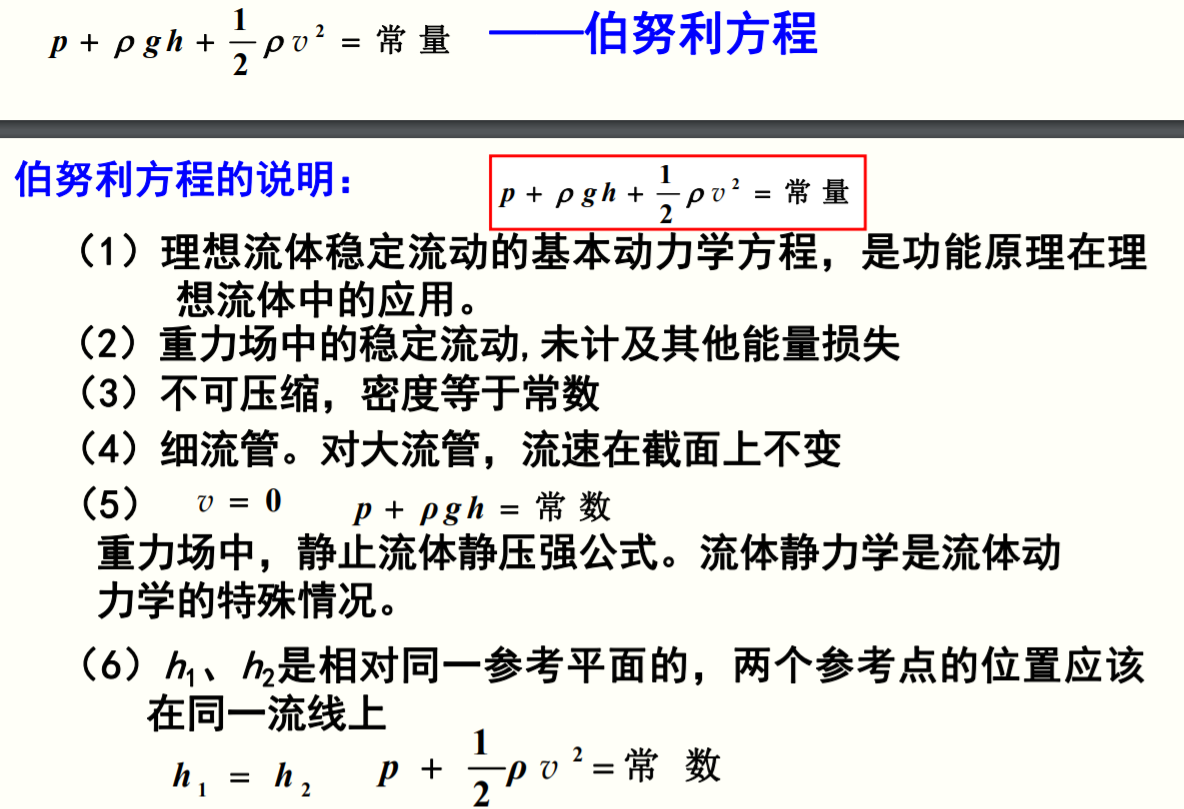
\includegraphics[width=13cm, height=12cm]{D:/UniversityNote/PhyNote/11.png}

\newpage
\section{第七讲\;\;相对论基础}
\subsection{洛伦兹变换}

\[ \mbox{洛伦兹坐标变换}\left\{
\begin{aligned}
x^{'} & = & \frac{x - vt}{\sqrt{1 - \frac{v^2}{c^2}}} \\
y^{'} & = & y \\
z^{'} & = & z \\
t^{'} & = & \frac{t - \frac{vx}{c^2}}{\sqrt{1 - \frac{v^2}{c^2}}}
\end{aligned}
\right.
\;\;\;\;\;
\mbox{洛伦兹坐标逆变换}\left\{
\begin{aligned}
x & = & \frac{x^{'} - vt}{\sqrt{1 - \frac{v^2}{c^2}}} \\
y & = & y^{'} \\
z & = & z^{'} \\
t & = & \frac{t^{'} - \frac{vx}{c^2}}{\sqrt{1 - \frac{v^2}{c^2}}}
\end{aligned}
\right.
\]
\[ \mbox{洛伦兹速度变换}\left\{
\begin{aligned}
u^{'}_x & = & \frac{u_x - v}{1 - \frac{vu_x}{c^2}} \\
u^{'}_y & = & \frac{u_y}{1 - \frac{vu_x}{c^2}}\sqrt{1 - \frac{v^2}{c^2}} \\
u^{'}_z & = & \frac{u_z}{1 - \frac{vu_x}{c^2}}\sqrt{1 - \frac{v^2}{c^2}}
\end{aligned}
\right.
\;\;\;
\mbox{洛伦兹速度逆变换}\left\{
\begin{aligned}
u_x & = & \frac{u^{'}_x - v}{1 + \frac{vu^{'}_x}{c^2}} \\
u_y & = & \frac{u^{'}_y}{1 + \frac{vu^{'}_x}{c^2}}\sqrt{1 - \frac{v^2}{c^2}} \\
u_z & = & \frac{u^{'}_z}{1 + \frac{vu^{'}_x}{c^2}}\sqrt{1 - \frac{v^2}{c^2}}
\end{aligned}
\right.
\]

\subsection{狭义相对论的时空观}

    同时的相对性:在不同的惯性参考系中观测,时间发生的顺序可能颠倒

    时间延缓效应:
    \[\Delta t = \frac{\Delta t_0}{\sqrt{1 - \frac{v^2}{c^2}}}\]

    长度收缩效应:
    \[L = L_0\sqrt{1 - \frac{v^2}{c^2}}\]

\subsection{相对论动力学基础}

    相对论质量,动量,能量的定义以及爱因斯坦质能关系
    \[m = \frac{m_0}{\sqrt{1 - v^2}c^2}\;\;\;p = \frac{m_0v}{\sqrt{1 - \frac{v^2}{c^2}}}\]

    \[E = mc^2\;\;\;E^2 = p^2c^2 + m_0^2c^4 = E_k + m_0c^2\]
\newpage
\section{第八讲\;\;简谐振动}
\subsection{简谐振动的定义}

    一、振动的定义及分类

    1.定义:一个物理量在某一定值附近往复变化,该物理量的运动形式成为振荡

    \;\;特征:存在平衡位置+具有周期性

    2.分类:按物理量类型划分:电磁振荡+机械振动

    \;\;在某一空间位置附近做来回往复的周期运动的物体做机械振动

    \;\;按受力或能量转换划分:自由振动(无阻尼振动,阻尼振动)+受迫振动

    根据机械振动的定义可知,机械振动的运动方程可以用周期函数来描述$f(t) = f(t+T)$

    任何一个复杂的振动均可分解为若干个以正(余)弦形式运动的振动
    \\

    二、简谐运动的定义

    1.定义:物体运动时,物体相对于平衡位置的位移按余弦(正弦)函数的规律随时间变化,这样的振动称为简谐振动,又称为谐振动。
    简谐运动是最简单、最基本的振动。

    2.模型:弹簧振子(线性谐振动)模型 = 轻弹簧 + 平动刚体

    3.运动方程:$x = Acos(\omega t + \phi_0)$,$A$振幅,$\omega$原频率,$\phi_0$初相位

\subsection{简谐运动的基本特征}

    一、两个理想化模型

    1.弹簧振子

    受力分析:$F = -kx$

    由牛顿第二定律,得:
    \[-kx = ma = m\frac{d^2x}{dt^2}\;\;\;\mbox{其中:}\frac{k}{m} = \omega^2\]

    动力学微分方程:
    \[\frac{d^2x}{dt^2} + \omega^2 x = 0\;\;\;\mbox{其中:}\frac{k}{m} = \omega^2\]

    运动学方程(振动方程):
    \[x = Acos(\omega t + \phi_0)\]

    2.单摆(小角度)

    受力分析:$M = -mgl\theta$

    由转动定律,有:
    \[M = J\beta = ml^2\frac{d^2\theta}{dt^2}\;\;\;\mbox{其中:}\frac{g}{l} = \omega^2\]

    动力学微分方程:
    \[\frac{d^2\theta}{dt^2} + \omega^2\theta = 0\;\;\;\mbox{其中:}\frac{g}{l} = \omega^2\]

    运动学方程(振动方程):
    \[\theta = \theta_0cos(\omega t + \phi_0)\]

    二、简谐运动的判定

    1.物体只受线性恢复力作用
    \[F = -kx\mbox{或}M= -k\theta\]

    2.动力学方程满足
    \[\frac{d^2x}{dt^2} + \omega^2x = o\]

    3.在无外来强迫力作用下,质点离开平衡位置的位移是时间的正弦函数或余弦函数
    \[x = Acos(\omega t + \phi_0)\]

    判断一振动是否是简谐振动用三种定义中任何一种皆可

    三、简谐运动的速度和加速度

    动力学方程:
    \[\frac{d^2x}{dt^2} = -\omega^2 x\]

    解方程得:
    \[x = Acos(\omega t + \phi)\;\;\;A,\phi\mbox{是积分常数,根据初始条件确定}\]

    速度:
    \[v = \frac{dx}{dt} = -A\omega sin(\omega t + \phi)\]

    加速度:
    \[a = \frac{d^2x}{dt^2} = -A\omega^2cos(\omega t + \phi) = -\omega^2x\]

\subsection{描述简谐运动的物理量}

    1.振幅A:与振动系统初始运动状态和系统属性有关,反应能量大小。
    \[A = \sqrt{x_0^2 + \frac{v_0^2}{\omega^2}}\]

    2.圆(角)频率$\omega$:由系统本身属性决定的常数,与初始条件无关(固有角频率)

    周期:$T = \frac{2\pi}{\omega}$,物体完成一次全振动所经历的时间,[SI]:s

    频率:$\nu = \frac{1}{T} = \frac{\omega}{2\pi}$,单位时间内质点完成的全振动的次数,[SI]:Hz

    角频率:$\omega = 2\pi\nu$,描述谐振运动的频率和周期,[SI]:$rad\cdot s^{-1}$

    3.相位$\omega t + \phi_0$,初相$\phi_0$

    (1)初相位:$\phi_0$,描述t=0时刻的运动状态
    \[\phi_0 = arctan(-\frac{v_0}{\omega x_0})\]

    (2)相位(位相)$\omega t + \phi$的物理意义:反应系统振动状态,运动状态变化趋势,比较频率相同的两振动系统的振动步调

\subsection{简谐运动的表示方法}

    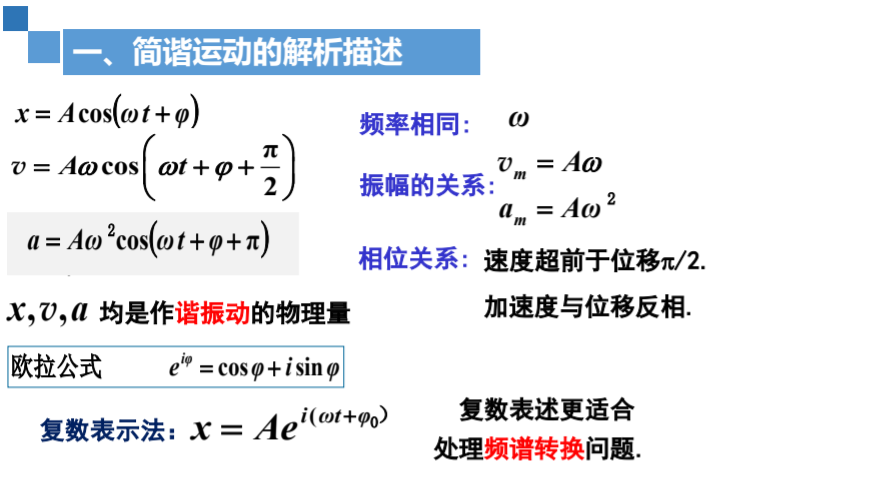
\includegraphics[width=13cm, height=8cm]{D:/UniversityNote/PhyNote/9/901.png}
    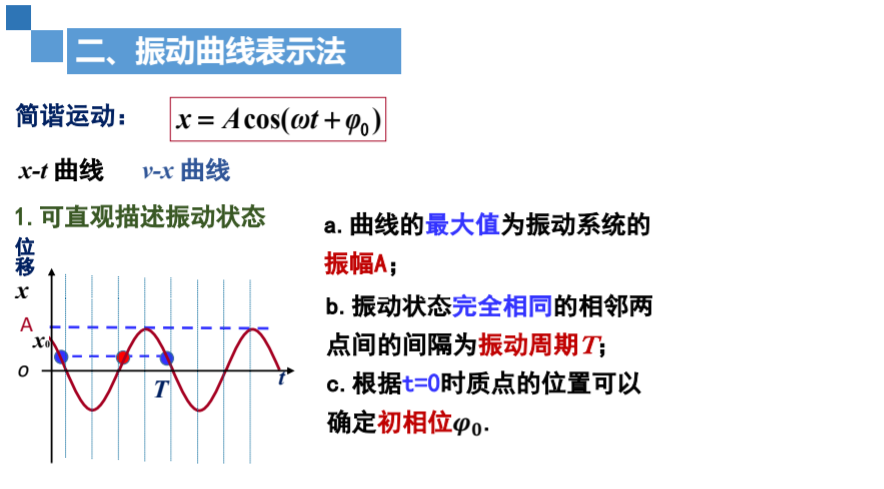
\includegraphics[width=13cm, height=8cm]{D:/UniversityNote/PhyNote/9/902.png}
    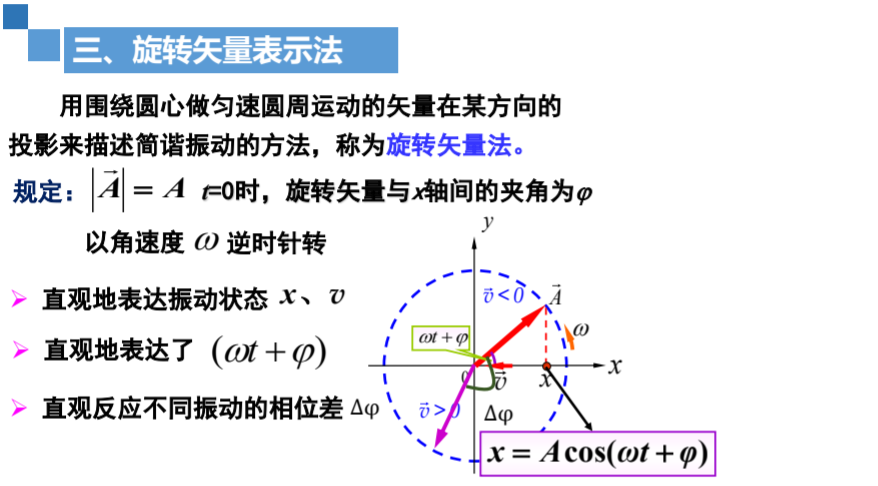
\includegraphics[width=13cm, height=8cm]{D:/UniversityNote/PhyNote/9/903.png}

\subsection{简谐运动的能量}

    1.谐振动系统的动能:
    \[E_k = \frac{1}{2}mv^2 = \frac{1}{2}m\omega^2 A^2sin^2(\omega t + \phi_0)\]

    2.谐振动系统的势能:
    \[E_p = \frac{1}{2}kx^2 = \frac{1}{2}kA^2cos^2(\omega t + \phi_o)\;\;\;\mbox{考虑到:}\frac{k}{m}\omega^2\]

    3.谐振动系统的总能量:
    \[\mbox{孤立谐振动系统机械能守恒:}E = E_k + E_p = \frac{1}{2}kA^2\]

    4.动能和势能的变化频率是位移变化频率的2倍,总能量并不改变。

    5.能量方法是工程中求振动系统固有频率是常用的方法:

    由振动过程中机械能守恒:
    \[E = \frac{1}{2}mv^2 + \frac{1}{2}kx^2 = \mbox{常数}\]

    两边求导:
    \[mv\frac{dv}{dt} + kx\frac{dx}{dt} = 0\Longrightarrow m\frac{d^2x}{dt^2} + kx = 0\Longrightarrow \omega^2 = \frac{k}{m}\]

\subsection{简谐运动的合成}
\subsubsection{同方向同频率简谐运动的合成}

    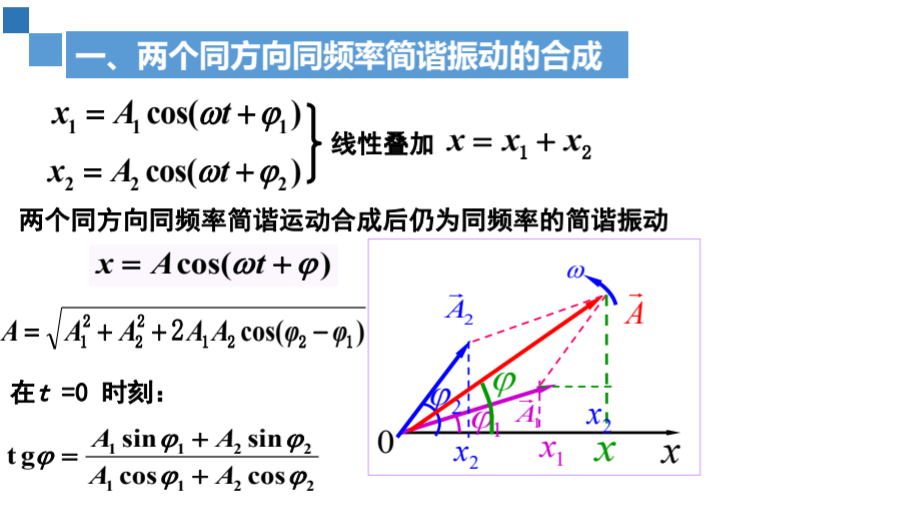
\includegraphics[width=13cm, height=8cm]{D:/UniversityNote/PhyNote/9/904.png}
    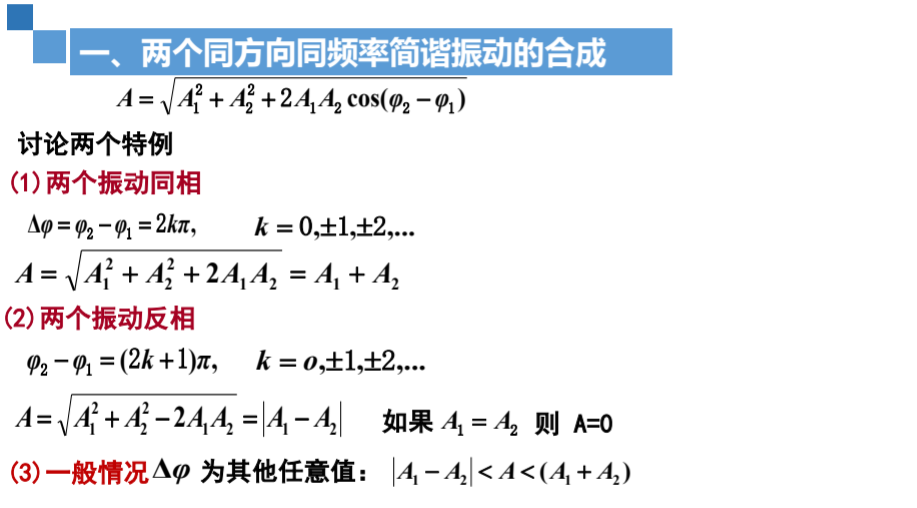
\includegraphics[width=13cm, height=8cm]{D:/UniversityNote/PhyNote/9/905.png}
    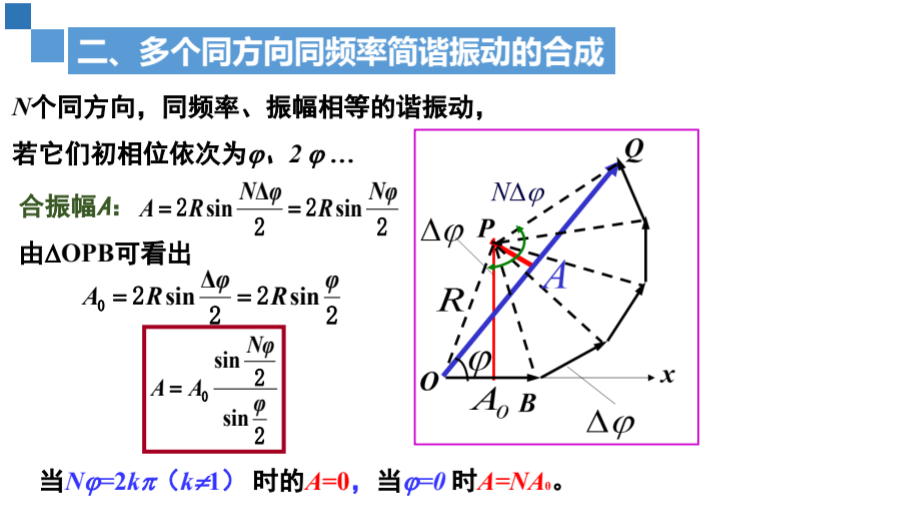
\includegraphics[width=13cm, height=8cm]{D:/UniversityNote/PhyNote/9/906.png}

\subsubsection{同方向不同频率简谐振动的合成}

    若$\omega_1 = \omega_2$,则$\Delta \phi$不变;同方向同频率两个简谐运动的合成仍为简谐运动

    若$\omega_1 \neq \omega_2$,则$\Delta \phi$变;同方向不同频率的两个简谐运动搞的合成为一复杂运动

    同方向不同频率简谐振动的合成:
    \[x_1 = Acos\omega_1 t\;\;\;x_2 = Acos\omega_2 t\mbox{振幅相同,初相为零}\]

    \[x = x_1 + x_2 = Acos\omega_1 t + Acos\omega_2 t = 2Acos\frac{(\omega_2 - \omega_1)t}{2}cos\frac{(\omega_2 + \omega_1)t}{2}\]

    当$\omega_1 - \omega_2<<\omega_1\; or \;\omega_2$时,振幅随时间的变化非常缓慢

    拍:频率较大而频率差较小的两个同方向简谐振动合成时,其和振动的振幅时而增强时而减弱的现象

    拍频:单位时间内合成振幅加强(减弱)的次数
    \[\nu_{\mbox{拍}} = \vert \frac{\omega_2 - \omega_1}{2\pi} \lvert = \vert \nu_2 - \nu_1 \lvert\]

\subsection{互相垂直的谐振动的合成}

    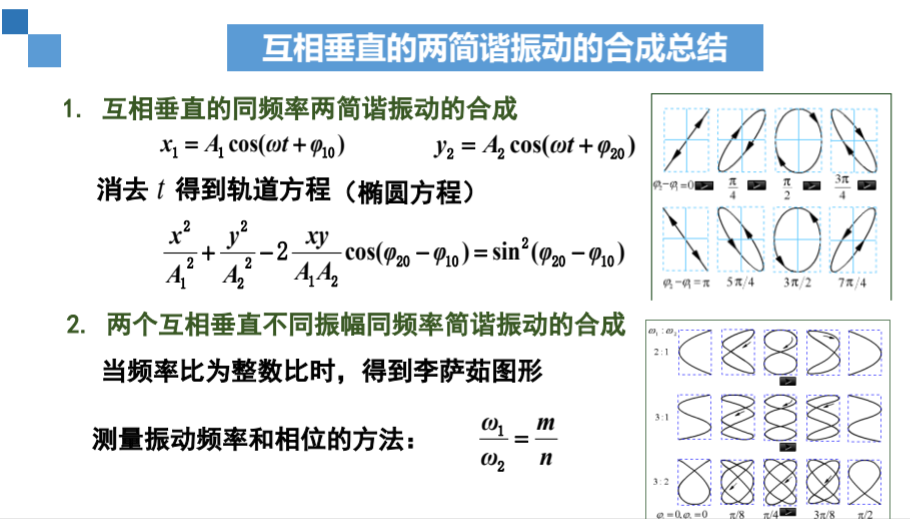
\includegraphics[width=13cm, height=8cm]{D:/UniversityNote/PhyNote/9/907.png}

\newpage
\section{第九讲\;\;机械波}
\subsection{机械波的基本属性}

    一、波的定义:波是自然界中一种常见的物质运动形式,波仅伴随着加载信息的能量传递

    质点运动:实体载着信息和能量运动,若干包含能量的小的物质集合的整体运动

    波的传播:信息和能量的传播,没有物质实体的移动,能量的扩展分布,充满其传播空间

    二、波的分类:

    1.机械波:机械振动在弹性介质中的传播,在介质中传播时受牛顿定律的支配

    2.电磁波:可以在真空中传播

    3.物质波:微观粒子具有波动性,反应概率密度的空间分布

    波的共同属性:都伴随能量传播,有反射、折射、干涉、衍射现象

    三、机械波的基本属性:机械振动(波源)在弹性介质(通过相互之间的弹性力组合在一起的连续介质)中的传播形成机械波。
    
    机械波产生条件:振源+弹性介质

    是运动状态的传播,弹性介质的质点并不随波传播.
    
    四、横波和纵波

    1.横波:质点振动方向与波的传播方向相垂直的波。特征:具有交替出现的波峰和波谷;仅在固体中传播

    2.纵波:质点振动方向与波的传播方向相平行的波。固、液、气体中均可传播

    横波和纵波都是行波

\subsection{机械波的描述}

    一、波线和波面

    波面:某时刻,同一波源向外传播的波到达的空间各点连成的面(同相位面)
    
    波阵面:波在传播过程中行进在最前面的波面,又称波前

    波(射)线:描述波传播的方向的射线。在各向均匀介质中波射线垂直于波面,波射线是波的能量传播方向

    根据波面的形状,可以将波分为:球面波(点源)、柱面波(线源)、平面波(面源)

    二、波函数与波动曲线

    波形图:$y = y(x,t)$,某时刻各点振动的位移y(广义:任一物理量)与相应的平衡位置坐标x的关系曲线

    三、机械波的特征量

    振幅:A\;\;质点偏离自身平衡位置所达到的最大正向位移

    波长:$\lambda$\;\;一个完整波形的长度。即:沿波的传播方向,两个相邻的、相位差为$2\pi$的振动质点之间的距离

    周期:T\;\;波前进一个波长的距离所需要的时间

    频率:单位时间内波动所传播的完整波的数目,$\nu = \frac{1}{T}$

    周期或频率只决定于波源的振动

    波速:u\;\;波动过程中,某一振动状态(即振动相位)单位时间内所传播的距离(相速)

    \[u = \frac{\lambda}{T} = \lambda\nu]\;\;\;\lambda = \frac{u}{\nu} = Tu\]

    波速只决定于媒质的性质

    固体内:横波\;$u = \sqrt{\frac{G}{\rho}}$,纵波\;$u = \sqcup\frac{E}{\rho}$

    液体、气体内:纵波\;$u = \sqrt{\frac{K}{\rho}}$

\subsection{平面间谐波波函数}

    一、平面间谐波

    1.平面简谐波定义:平面波传播过程中,若介质中各质元均做同振幅、同频率的简谐振动,该波称为平面简谐波

    2.平面简谐波产生条件:作简谐运动的波源\;+\;均匀无吸收的弹性介质

    3.平面简谐波是最基本、最简单的波动形式,复杂波可看成是不同频率简谐波叠加的结果

    二、平面简谐波波函数

    反映平面简谐波在均匀介质中传播时,介质中各质元相对于自身平衡位置的位移随时间的变化的函数。任一波线上各点的振动状态可代表整个波的状态

    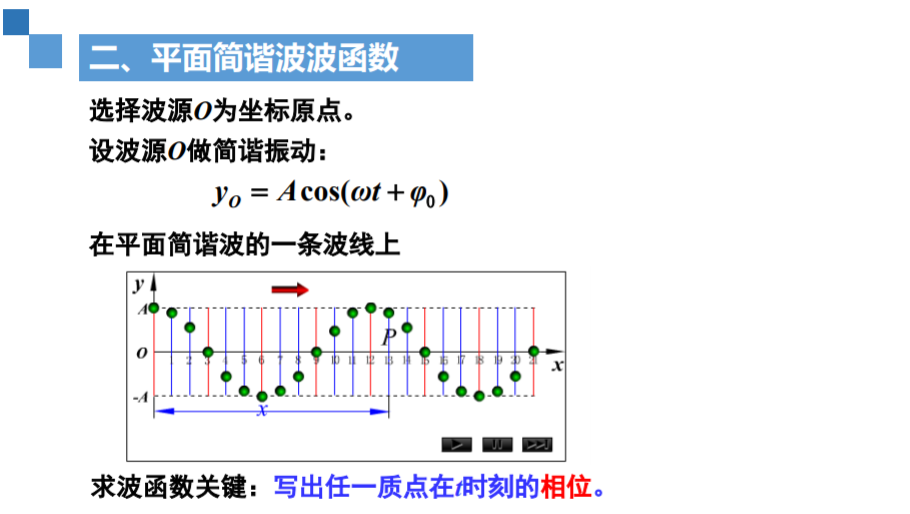
\includegraphics[width=13cm, height=8cm]{D:/UniversityNote/PhyNote/10/1001.png}
    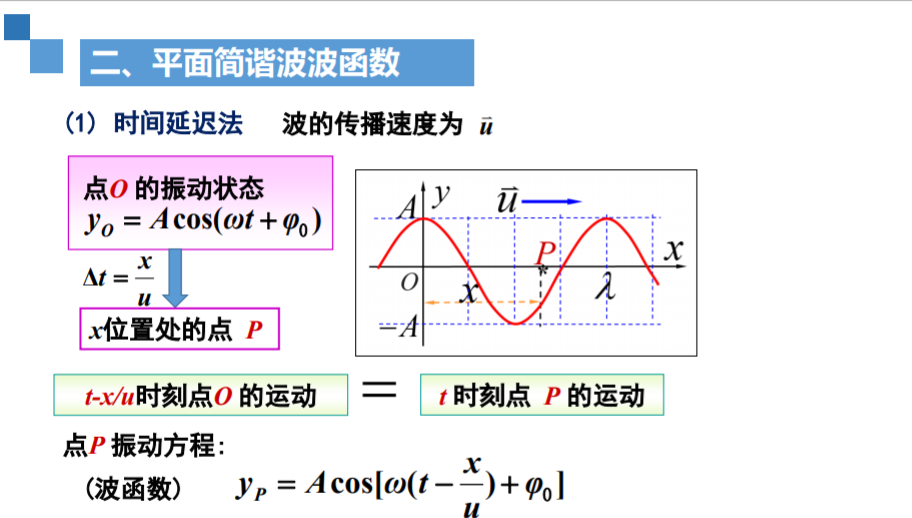
\includegraphics[width=13cm, height=8cm]{D:/UniversityNote/PhyNote/10/1002.png}
    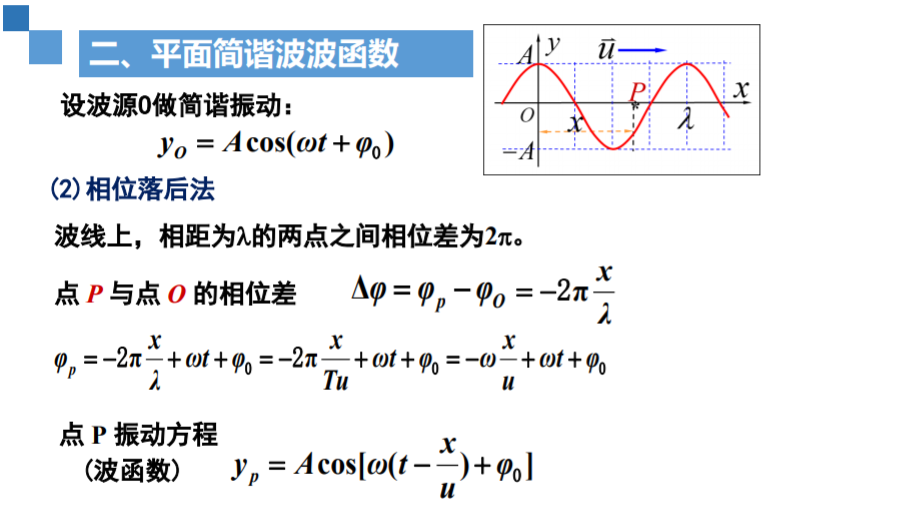
\includegraphics[width=13cm, height=8cm]{D:/UniversityNote/PhyNote/10/1003.png}
    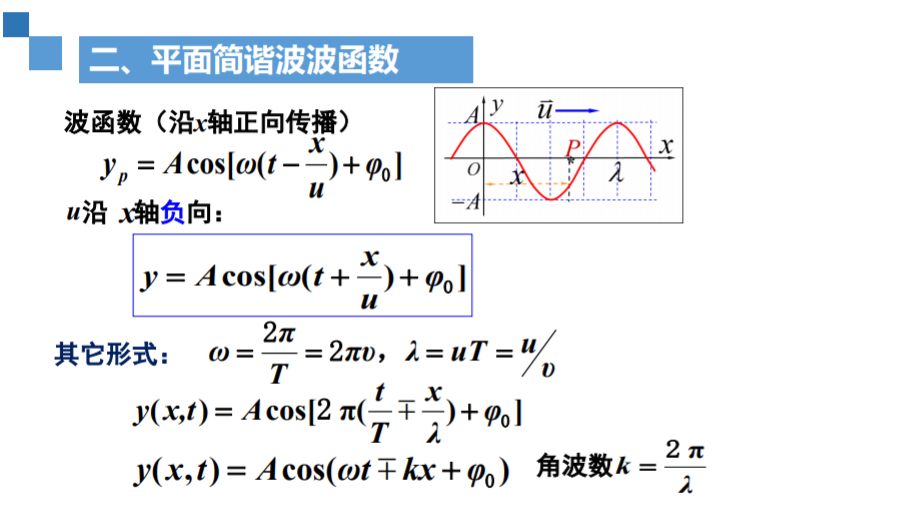
\includegraphics[width=13cm, height=8cm]{D:/UniversityNote/PhyNote/10/1004.png}
    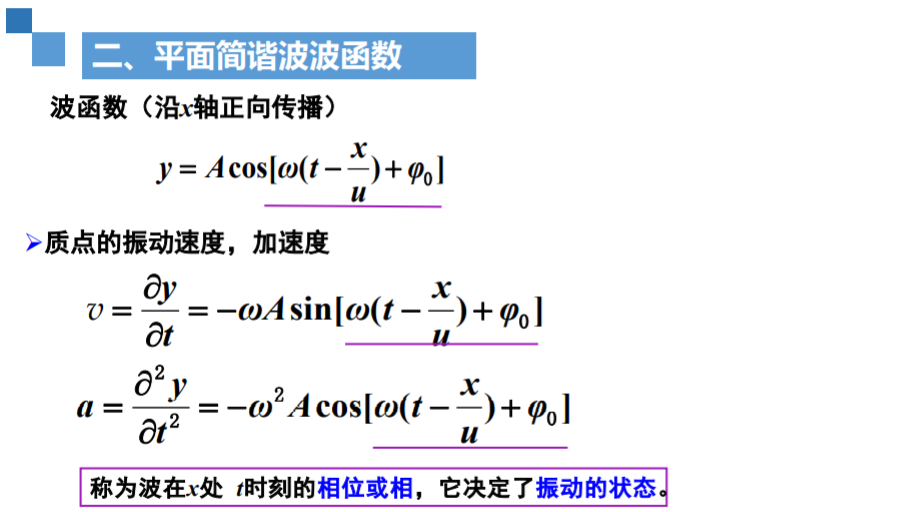
\includegraphics[width=13cm, height=8cm]{D:/UniversityNote/PhyNote/10/1005.png}

    波函数(沿x轴正向传播):$y = Acos[\omega(t - \frac{x}{u}) + \phi_0]$

    对于某一给定的相位
    \[\omega (t - \frac{x}{u}) = \mbox{常量}\phi\]

    两边对t求导可得相位的传播速度
    \[\frac{dx}{dt} = u\]

    说明波的相位的传播速度就是波的速度u,所以波速u也称为相速度,它可以超过光速

\subsection{波函数的物理意义和波动方程}

    一、波函数的物理意义
    \[y = Acos[\omega(t - \frac{x}{u} + \phi_0)] = Acos[2\pi(\frac{t}{T} - \frac{x}{\lambda}) + \phi_0]\]

    1.x固定时,表示该点的振动方程,体现波的时间周期性

    2.当t一定时,表示该时刻波线上各点相对其平衡位置的位移,体现波的空间周期性

    3.若x、t均变化,表示波形沿传播方向的运动情况(行波)

    二、波动方程
    \[y = Acos[\omega(t - \frac{x}{u} + \phi_0)]\]

    对变量二次求导
    \[\frac{\partial^2y}{\partial t^2} = -\omega^2Acos[\omega(t - \frac{x}{u} + \phi_0)]\]
    \[\frac{\partial^2y}{\partial x^2} = -\frac{\omega^2}{u^2}Acos[\omega(t - \frac{x}{u} + \phi_0)]\]

    波动微分方程
    \[\frac{\partial^2y}{\partial x^2} = \frac{1}{u^2}\frac{\partial^2y}{\partial t^2}\]

    具有普适性,即对任意一维平面波都成立

\subsection{机械波的能量}

    一、波动能量的传播

    以固体棒中传播的纵波为例分析波动能量的传播

    波函数:$y = Acos\omega(t - \frac{x}{u})$,介质密度为$\rho$

    振动动能:
    \[dW_k = \frac{1}{2}(dm)v^2 = \frac{1}{2}(\rho dV)v^2 = \frac{1}{2}\rho dVA^2\omega^2sin^2\omega(t - \frac{x}{u})\]

    弹性势能:
    \[dW_p = \frac{1}{2}k(dy)^2 = \frac{1}{2}\rho dVA^2\omega^2sin^2\omega (t - \frac{x}{u})\]

    \[dW_k = dW_p = \frac{1}{2}\rho dVA^2\omega^2sin^2\omega(t - \frac{x}{u})\]

    体积元的总机械能:
    \[dW = dW_k + dW_p = \rho dVA^2\omega^2sin^2\omega(t - \frac{x}{u})\]

    1. 传播的媒质中,任一质元的动能、势能、总机械能均作同相位的周期性变化

    \;\;平衡位置时,三者均最大

    \;\;位移最大时,三者均为零

    2. 传播的媒质中,任一质元不断地传播能量,机械能不守恒

    3. 传播的媒质中,质元做的是受迫振动,而非简谐振动

    能量密度:单位体积介质中的波动能量
    \[w = \frac{dW}{dV} = \rho A^2\omega^2sin^2\omega(t - \frac{x}{u})\]

    平均能量密度:能量密度在一个周期内的平均值
    \[\overline{w} = \frac{1}{T}\int_0^Twdt = \frac{1}{2}\rho\omega^2 A^2\]

    能流:单位时间通过介质中某一面积的能量
    \[p = \frac{wSudt}{dt} = wSu\]

    平均能流:能流在一个周期内的时间平均值
    \[\overline{P} = \overline{w}uS\]

    平均能流密度(波的强度)I:通过与波传播方向垂直的单位
    面积的平均能流
    \[I = \frac{\overline{P}}{S} = \overline{w}u\Rightarrow I = \frac{1}{2}\rho A^2\omega^2u\]

\subsection{波的衍射\;\;惠更斯原理}

    一、波的衍射

    波传播遇到障碍物时,波的传播方向偏离原来直线传播方向的现象称为衍射。一切波动都具有衍射现象,衍射是波动的直接证据之一

    衍射特点:障碍物(受限)的尺度与波长相接近时,能够观察到明显的衍射现象

    二、惠更斯原理

    在波的传播过程中,波前上每一点都可以看作是发射子波的波源,而在其后的任意时刻,这些子波的包络面就是新的波前

    原理依据: 
    
    \;\;1. 波动在介质是逐点传播;

    \;\;2. 波动是振动状态的传播。同一波前上所有子波源的振动状态完全相同,因此,其后任意时刻各子波都具有相同的相位  

    衍射的实质是波面破损或畸变

    惠更斯原理的局限性:无法说明子波强度的分布和子波不向后传播的问题

    三、惠更斯——菲涅耳原理

    波前(波阵面)上每个面元都可以看成是发出球面子波的波源;各子波在空间某点的相干叠加,就决定了该点波的强度。原理的核心是子波相干叠加

\subsection{波的反射和折射}

    一、反射定律

    1.反射线、入射线和界面的法线在同一平面内

    2.$i = i^{'}$

    二、折射定律

    1.折射线、入射线和界面的法线在同一平面内

    2.$\frac{sin i}{sin r} = \frac{u_1}{u_2}$

\subsection{波的干涉}

    一、波的叠加原理

    几列波相遇之后,仍然保持它们各自原有的特征(频率、波长、振幅、振动方向等)不变,并按照原来的方向继续前进,好象没有遇到过其他波一样。在相遇区域内任一点的振动,为各列波单独存在时在该点所引起的振动位移的矢量和。仅在波动方程为线性方程(波强不太大)时成立

    二、波的干涉

    两列相干波相遇时,使某些地方振动始终加强,而使另一些地方振动始终减弱的现象,称为波的干涉现象。(波强的非均匀稳定分布)

    相干波的条件:

    \;\;1.频率相同

    \;\;2.振动方向平行或同一方向有分量

    \;\;3.相位相同或相位差恒定
    \[A = \sqrt{A_1^2 = A_2^2+ 2A_1A_2cos\Delta\phi}\;\;\Delta\phi = \phi_2 - \phi_1 - \frac{2\pi}{\lambda}\delta\]

    波程差:$\delta = r_2 - r_1$

    $\delta = \pm k\lambda\;\;k = 0, 1, 2,\dots\;\;A = A_1 + A_2$\;\;振动始终加强

    $\delta = \pm(k + \frac{1}{2})\lambda\;\;k = 0, 1, 2,\dots\;\;A = \vert A_1 - A_2\lvert $\;\;振动始终减弱

    $\delta = \mbox{其他}\;\;\vert A_1 - A_2 \lvert < A < A_1 + A_2$

\subsection{半波损失}

    一、驻波的产生

    振幅都相同的两列相干波,在同一直线上沿相反方向传播时,某些点的合振幅始终为零(波节),某些点的合振幅始终最大(波腹),这种特殊的干涉现象就称为驻波

    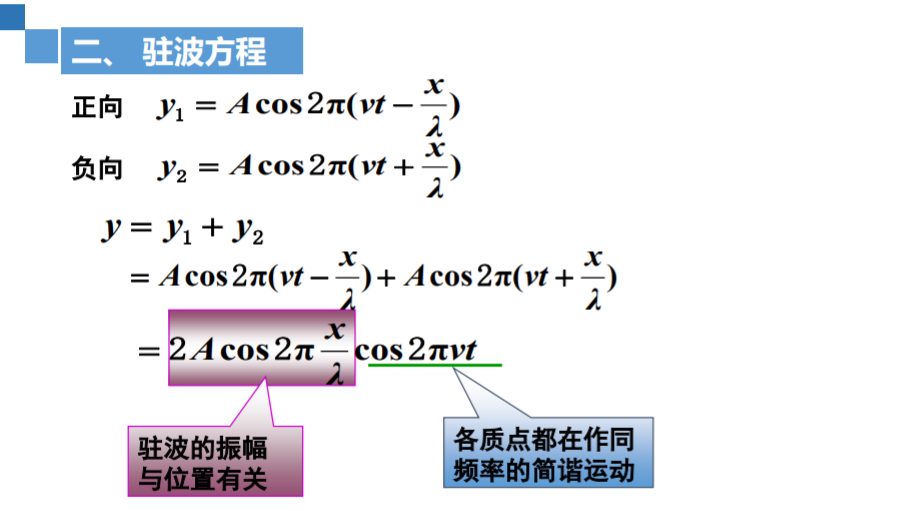
\includegraphics[width=13cm, height=8cm]{D:/UniversityNote/PhyNote/10/1006.png}
    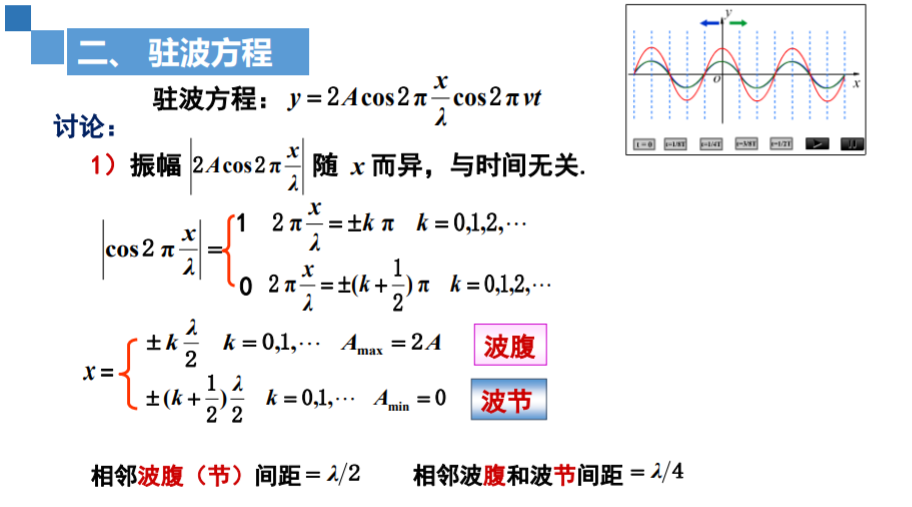
\includegraphics[width=13cm, height=8cm]{D:/UniversityNote/PhyNote/10/1007.png}
    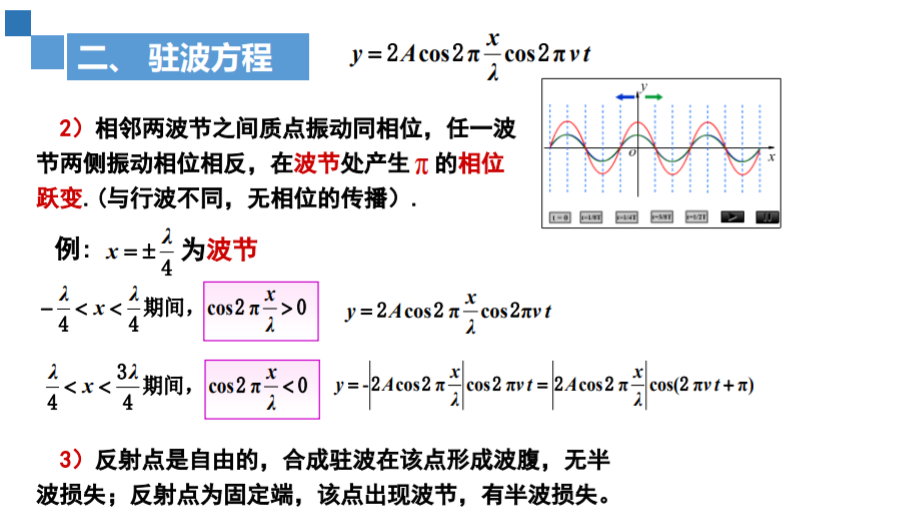
\includegraphics[width=13cm, height=8cm]{D:/UniversityNote/PhyNote/10/1008.png}
    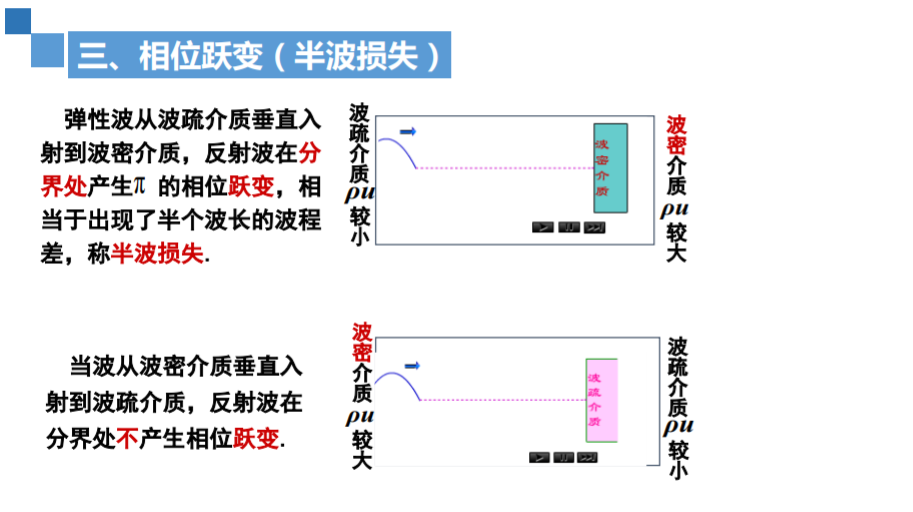
\includegraphics[width=13cm, height=8cm]{D:/UniversityNote/PhyNote/10/1009.png}
    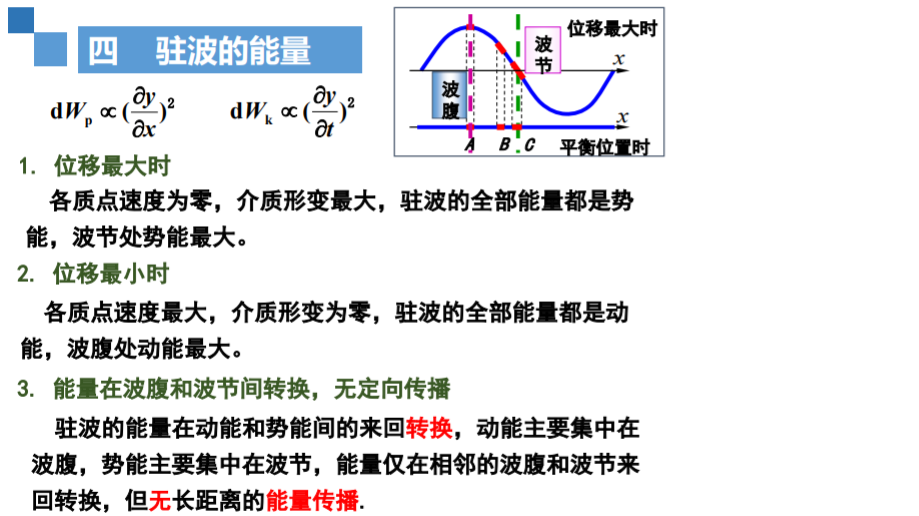
\includegraphics[width=13cm, height=8cm]{D:/UniversityNote/PhyNote/10/1010.png}

\subsection{多普勒效应}

    1. 多普勒效应定义
    
    若波源或观察者,或两者同时相对介质运动,则观察者接收到的的频率和波源的振动频率不同的现象,称为多普勒效应

    2. 机械波的多普勒效应
    \[\nu^{'} = \frac{u\pm v_0cos\beta}{u\pm v_s cos\alpha}\nu\]
    其中:
    
    $\nu$波源振动的频率;$\nu^{'}$:探测器探测的频率;$u$:波相对于介质的速度;$v_0$:探测器相对于介质的速度;$v_s$:波源相对于介质的速度


    3. 电磁波的多普勒效应
    光源和接收器在同一直线上运动时,考虑相对论效应:
    \[\nu^{'} = \sqrt{\frac{c + v}{c - v}\nu}\]

    v是光源和接收器的相对运动速度

    两者相向运动时,接收波长变短,这种现象称为“紫移”。光源和接收器相背运动时,接收波长变长,这种现象称为“红移”
    
\end{document}
\end{document}